\documentclass[]{report}

% Define page
\usepackage[top=1in, bottom=1in, left=1in, right=1in]{geometry}
\linespread{1.1}

% For math
\usepackage{amsmath,amsthm,amssymb}
\usepackage{bm}

% For figures
\usepackage{graphicx,subfigure,psfrag,epsfig}
\graphicspath{{images/}}

% Url's and clickable pdf
\usepackage[dvips,breaklinks,bookmarks,bookmarksnumbered]{hyperref}
\hypersetup{
  pdftitle={elastix, the manual},
  pdfauthor={Stefan Klein and Marius Staring},
  colorlinks={true},      % false: boxed links; true: colored links
  linkcolor=red,          % color of internal links
  citecolor=green,        % color of links to bibliography
  filecolor=magenta,      % color of file links
  urlcolor=cyan           % color of external links
}
\usepackage{url,breakurl}

\usepackage{natbib}
\usepackage{ctable}

% Definitions
\newcommand{\elastix}{\texttt{elastix}}
\newcommand{\transformix}{\texttt{transformix}}
\newcommand{\etal}{\emph{et al.}}
\newcommand{\vx}{\bm{x}}
\newcommand{\vxt}[1][]{\bm{\widetilde x}_{#1}}
\newcommand{\vu}{\bm{u}}
\newcommand{\vux}{\bm{u}(\bm{x})}
\newcommand{\vmu}{\bm{\mu}}
\newcommand{\vT}{\bm{T}}
\newcommand{\vTm}{\bm{T}_{\vmu}}
\newcommand{\vTmx}{\bm{T}_{\vmu}(\bm{x})}
\newcommand{\CC}{\mathcal{C}}
\newcommand{\Ncal}{\mathcal{N}}
\newcommand{\Sim}{\mathcal{S}}
\newcommand{\Pen}{\mathcal{P}}
\newcommand{\D}[2]{\frac{\partial #1}{\partial #2}}
\newcommand{\Dd}[3]{\frac{\partial^2 #1}{\partial #2 \partial #3}}

% see page474 latex manual:
\newcommand\relphantom[1]{\mathrel{\phantom{#1}}}

%%%%%%%%%%%%%%%%%%%%%%%%%%%%%%%%%%%%%%%%%%%%%%%%%%%%%%%%%%%%%%%%%%%%%%%%%%%%%%%%%%%%%%%%%%%%

\begin{document}

\title{
\includegraphics[width=8cm]{elastixLogo.eps}\\\vspace{1cm}the manual\vspace{1cm}}
\author{Stefan Klein and Marius Staring}
%\date{}
\maketitle

\setcounter{page}{1} \pagenumbering{roman} \tableofcontents
%\newpage
%\listoffigures
%\newpage
%\listoftables
\newpage
\pagenumbering{arabic} \setcounter{page}{1}

%%%%%%%%%%%%%%%%%%%%%%%%%%%%%%%%%%%%%%%%%%%%%%%%%%%%%%%%%%%%%%%%%%%%%%%%%%%%%%%%%%%%%%%%%%%%
% main text

\chapter{Introduction}\label{chp:Introduction}

This manual describes a software package for image registration:
\elastix. The software consists of a collection of algorithms that
are commonly used to solve medical image registration problems. A
large part of the code is based on the Insight Toolkit (ITK). The
modular design of \elastix\ allows the user to quickly test and
compare different registration methods for his/her specific
application. The command-line interface simplifies the processing
of large amounts of data sets, using scripting.

\section{Outline of this manual}

In Chapter~\ref{chp:Registration} quite an extensive introduction to
some general theory of image registration is given. Also, the
different components of which a registration method consists, are
treated. In Chapter~\ref{chp:elastix}, \elastix\ is described and
its usage is explained. Chapter~\ref{chp:transformix} is dedicated
to \transformix, a program accompanying \elastix. A tutorial is
given in Chapter~\ref{chp:Tutorial}, including many recommendations
based on the authors' experiences. More advanced registration topics
are covered in Chapter \ref{chp:advanced}. The final chapter
provides more details for those interested in the setup of the
source code and gives information on how to implement your own
additions to \elastix. In the Appendices \ref{chp:ExampleParam} and
\ref{chp:ExampleTransformParam} example (transform) parameter files
are given. Appendix \ref{chp:License} contains the software license
and disclaimer under which \elastix\ is currently distributed.

%Chapter~\ref{chp:develop} provides more details about the source code
%and explains how to create extensions of \elastix.

\section{Quick start}

\begin{itemize}
\item Download \elastix\ from \url{http://elastix.isi.uu.nl/download.php}.
    See Section \ref{sec:elastix:install} for details about the
    installation. Do not forget to subscribe to the \elastix\ mailing list,
    which is the main forum for questions and announcements.

\item Read some basics about the program at
    \url{http://elastix.isi.uu.nl/about.php} and in this manual.

\item Try the example of usage. It can be found in the \emph{About}
section of the website. If you don't get the example running at your
computer take a look at the FAQ in the general section:
\begin{quote}
\url{http://elastix.isi.uu.nl/FAQ.php}
\end{quote}

\item Read the complete manual if you are the type of person that
first wants to know.

\item Get started with your own application. If you need more information
    at this point you can now start reading the manual. You can find more
    information on tuning the parameters in Chapter \ref{chp:Tutorial}. A
    list of all available parameters can be found at
    \url{http://elastix.isi.uu.nl/doxygen/pages.html}. Also take a look at
    the \emph{parameter file database} at
    \url{http://elastix.isi.uu.nl/wiki.php}, for many example parameter
    files.

\item When you are stuck, don't miss the tutorial in Chapter
\ref{chp:Tutorial} of this manual. Also, take a look at the FAQ again
for some common problems.

\item When you are still stuck, do not hesitate to send an e-mail to the
    \elastix\ mailing list. In general, you will soon get an answer.
\end{itemize}

\section{Acknowledgements}

This manual has mainly been written while the authors worked at the Image
Sciences Institute (ISI, \url{http://www.isi.uu.nl}), Utrecht, The Netherlands.
We thank the users of \elastix, whose questions and remarks helped improving
the usability and documentation of \elastix. Specifically, we want to thank the
following people for proofreading (parts of) this manual when we constructed a
first version: Josien Pluim, Keelin Murphy, Martijn van der Bom, Sascha
M\"{u}nzing, Jeroen de Bresser, Bram van Ginneken, Kajo van der Marel,
Adri\"{e}nne Mendrik (in no specific order).

%%%%%%%%%%%%%%%%%%%%%%%%%%%%%%%%%%%%%%%%%%%%%%%%%%%%%%%%%%%%%%%%%%%%%%%%%%%%%%%%%%%%%%%%%%%%

\chapter{Image registration}\label{chp:Registration}

This chapter introduces primary registration concepts that are at
the base of \elastix. More advanced registration topics are covered
in Chapter \ref{chp:advanced}.

Image registration is an important tool in the field of medical
imaging. In many clinical situations several images of a patient
are made in order to analyse the patient's situation. These images
are acquired with, for example, X-ray scanners, Magnetic Resonance
Imaging (MRI) scanners, Computed Tomography (CT) scanners, and
Ultrasound scanners, which provide knowledge about the anatomy of
the subject. Combination of patient data, mono- or multi-modal,
often yields additional clinical information not apparent in the
separate images. For this purpose, the spatial relation between
the images has to be found. Image registration is the task of
finding a spatial one-to-one mapping from voxels in one image to
voxels in the other image, see Figure \ref{fig:concept}. Good
reviews on the subject are given in
\citet{MaintzEA98,LesterEA99,HillEA01,Hajnal01,Zit03:Image,
Modersitzki04:Numerical}.

The following section introduces the mathematical formulation of
the registration process and gives an overview of the components
of which a general registration method consists. After that, in
Sections~\ref{sec:comp:metric}-\ref{sec:comp:multiresolution},
each component is discussed in more detail. For each component,
the name used by \elastix\ is given, in \texttt{typewriter} style.
In Section~\ref{sec:evaluation}, methods to evaluate the
registration results are discussed.

\section{Registration framework}\label{sec:framework}

\begin{figure}
\centering
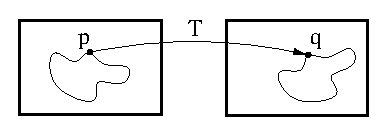
\includegraphics[width=8cm]{ImageRegistrationConcept.eps}
\caption{Image registration is the task of finding a spatial
transformation mapping one image to another. Adopted from
\citet{ITKSoftwareGuideSecondEdition}.} \label{fig:concept}
\end{figure}

Two images are involved in the registration process. One image, the
\emph{moving image} $I_M(\vx)$, is deformed to fit the other image,
the \emph{fixed image} $I_F(\vx)$. Registration is the problem of
finding a \emph{displacement} $\vux$ that makes $I_M(\vx + \vux)$
spatially aligned to $I_F(\vx)$. An equivalent formulation is to say
that registration is the problem of finding a \emph{transformation}
$\vT(\vx) = \vx + \vux $ that makes $I_M(\vT(\vx))$ spatially aligned
to $I_F(\vx)$. The quality of alignment is defined by a distance or
similarity measure $\Sim$, such as the sum of squared differences
(SSD), the correlation ratio, or the mutual information (MI) measure.
Because this problem is ill-posed for nonrigid transformations $\vT$,
a regularisation or penalty term $\Pen$ is often introduced that
constrains $\vT$.

Commonly, the registration problem is formulated as an optimisation
problem in which the cost function $\mathcal{C}$ is minimised w.r.t.
$\vT$:
\begin{align}
\hat \vT &= \arg \min_{\vT} \CC (\vT; I_F,I_M), \qquad \text{with} \label{eq:registration1}\\
\CC(\vT; I_F,I_M) &= -\Sim(\vT; I_F,I_M) + \gamma
\Pen(\vT),\label{eq:registration2}
\end{align}
where $\gamma$ weighs similarity against regularity. To solve the above
minimisation problem, there are basically two approaches: parametric and
nonparametric. The reader is referred to \cite{Fis04:Unified} for an overview
on nonparametric methods, which are not discussed in this manual. The \elastix\
software is based on the parametric approach. In parametric methods, the number
of possible transformations is limited by introducing a parametrisation (model)
of the transformation. The original optimisation problem thus becomes:
\begin{align}
\hat\vTm &= \arg \min_{\vTm}
 \CC(\vTm ; I_F,I_M), \label{eq:towardsparametric}
\end{align}
where the subscript $\vmu$ indicates that the transform has been
parameterised. The vector $\vmu$ contains the values of the
``transformation parameters''. For example, when the
transformation is modelled as a 2D rigid transformation, the
parameter vector $\vmu$ contains one rotation angle and the
translations in $x$ and $y$ direction. We may write Equation
(\ref{eq:towardsparametric}) also as:
\begin{align}
\hat\vmu &= \arg \min_{\vmu} \CC(\vmu; I_F,I_M).
\label{eq:parametric}
\end{align}
From this equation it becomes clear that the original problem
(\ref{eq:registration1}) has been simplified. Instead of optimising
over a ``space of functions $\vT$'', we now optimise over the
elements of $\vmu$. Examples of other transformation models are given
in Section~\ref{sec:comp:transform}.

\begin{figure}
\centering
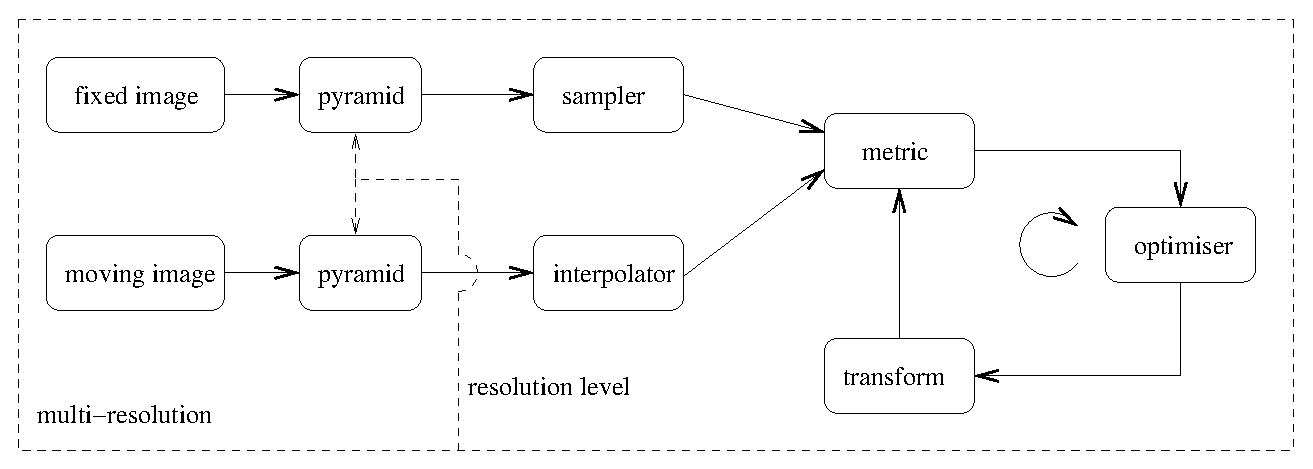
\includegraphics[width=\textwidth]{images/registrationcomponents.eps}
\caption{The basic registration components.}
\label{fig:registrationcomponents}
\end{figure}

Figure~\ref{fig:registrationcomponents} shows the general components
of a parametric registration algorithm in a block scheme. The scheme
is a slightly extended version of the scheme introduced in
\cite{ITKSoftwareGuideSecondEdition}. Several components can be
recognised from Equations
(\ref{eq:registration1})-(\ref{eq:parametric}); some will be
introduced later. First of all, we have the images. The concept of
an image needs to be defined. This is done in
Section~\ref{sec:comp:image}. Then we have the cost function $\CC$,
or ``metric'', which defines the quality of alignment. As mentioned
earlier, the cost function consists of a similarity measure $\Sim$
and a regularisation term $\Pen$. The regularisation term $\Pen$ is
not discussed in this chapter, but in Chapter \ref{chp:advanced}.
The similarity measure $\Sim$ is discussed in
Section~\ref{sec:comp:metric}. The definition of the similarity
measure introduces the sampler component, which is treated in
Section~\ref{sec:comp:sampler}. Some examples of transformation
models $\vT_{\vmu}$ are given in Section~\ref{sec:comp:transform}.
The optimisation procedure to actually solve the problem
(\ref{eq:parametric}) is explained in Section
\ref{sec:comp:optimiser}. During the optimisation, the value
$I_M(\vT_{\vmu}(\vx))$ is evaluated at non-voxel positions, for
which intensity interpolation is needed. Choices for the
interpolator are described in Section \ref{sec:comp:interpolator}.
Another thing, not immediately clear from Equations
(\ref{eq:registration1})-(\ref{eq:parametric}), is the use of
multi-resolution strategies to speed-up registration, and to make it
more robust, see Section \ref{sec:comp:multiresolution}.

\section{Images}\label{sec:comp:image}

Since image registration is all about images, we have to be
careful with what is meant by an image. We adopt the notion of an
image from the Insight Toolkit \citep[p.
40]{ITKSoftwareGuideSecondEdition}:

\begin{quote}
Additional information about the images is considered mandatory.
In particular the information associated with the physical spacing
between pixels and the position of the image in space with respect
to some world coordinate system are extremely important. Image
origin and spacing are fundamental to many applications.
Registration, for example, is performed in physical coordinates.
Improperly defined spacing and origins will result in inconsistent
results in such processes. Medical images with no spatial
information should not be used for medical diagnosis, image
analysis, feature extraction, assisted radiation therapy or image
guided surgery. In other words, medical images lacking spatial
information are not only useless but also hazardous.

Figure \ref{fig:image} illustrates the main geometrical concepts
associated with the itk::Image. In this figure, circles are used
to represent the centre of pixels. The value of the pixel is
assumed to exist as a Dirac Delta Function located at the pixel
centre. Pixel spacing is measured between the pixel centres and
can be different along each dimension. The image origin is
associated with the coordinates of the first pixel in the image. A
pixel is considered to be the rectangular region surrounding the
pixel centre holding the data value. This can be viewed as the
Voronoi region of the image grid, as illustrated in the right side
of the figure. Linear interpolation of image values is performed
inside the Delaunay region whose corners are pixel centres.
\end{quote}

\begin{figure}
\centering
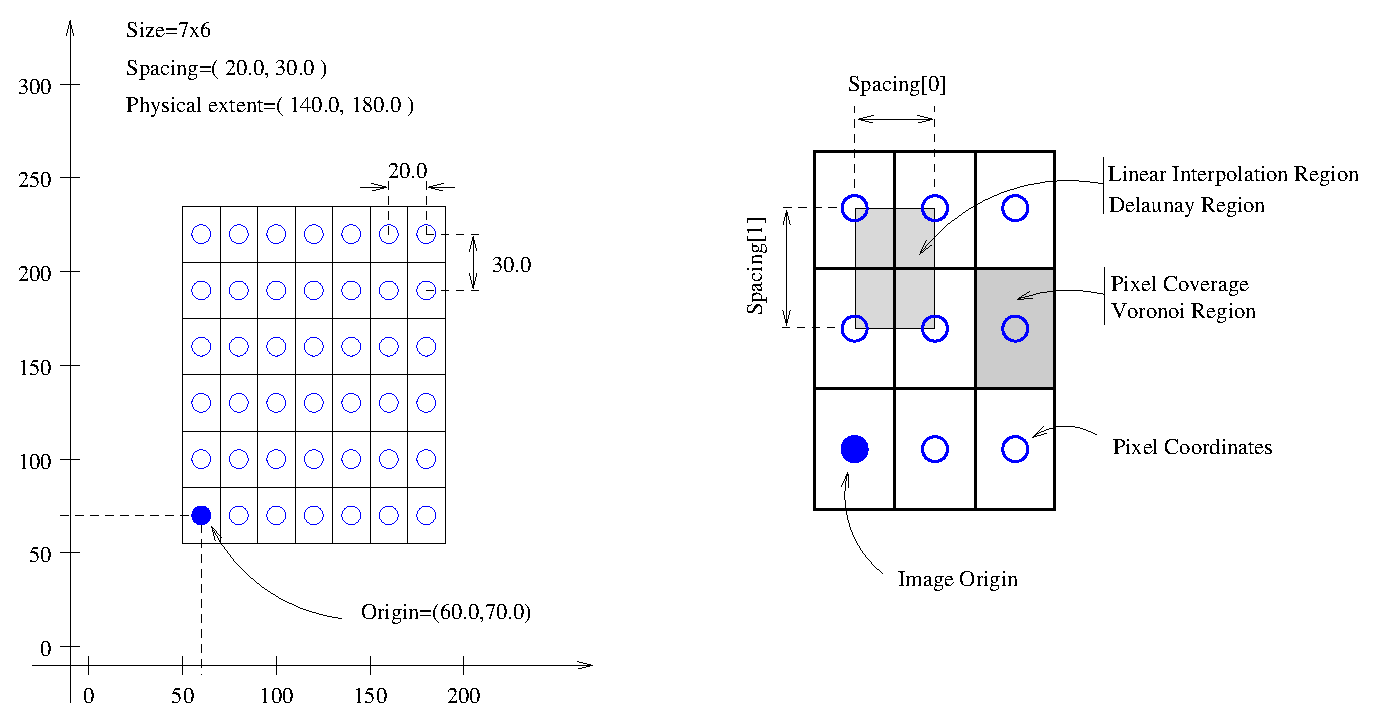
\includegraphics[width=12cm]{ImageOriginAndSpacing.eps}
\caption{Geometrical concepts associated with the ITK image.
Adopted from \citet{ITKSoftwareGuideSecondEdition}.}
\label{fig:image}
\end{figure}

Therefore, you should take care that you use an image format that
is able to store the relevant information (e.g. \texttt{mhd},
DICOM). Some image formats, like \texttt{vpx}, do not store the
origin and spacing. This may cause serious problems!

Up to \elastix\ version 4.2, the image orientation (direction
cosines) was not yet fully supported in \elastix. From \elastix\
4.3, image orientation is fully supported, but can be disabled for
backward compatibility reasons.

\section{Metrics}\label{sec:comp:metric}

Several choices for the similarity measure can be found in the
literature. Some common choices are described below. Between brackets
the name of the metric in \elastix\ is given:

\begin{description}
\item[Sum of Squared Differences (SSD):] (\texttt{AdvancedMeanSquares})
The SSD is defined as:
\begin{align}
\mathrm{SSD}(\vmu;I_F,I_M) &= \frac{1}{|\Omega_F|}
\sum\limits_{\vx_i \in \Omega_F} \left( I_F(\vx_i) -
I_M(\vT_{\vmu}(\vx_i)) \right)^2,\label{eq:ssd}
\end{align}
with $\Omega_F$ the domain of the fixed image $I_F$, and
$|\Omega_F|$ the number of voxels. Given a transformation $\vT$,
this measure can easily be implemented by looping over the voxels
in the fixed image, taking $I_F(\vx_i)$, calculating
$I_M(\vT_{\vmu}(\vx_i))$ by interpolation, and adding the squared
difference to the sum.

\item[Normalised Correlation Coefficient (NCC):]
(\texttt{AdvancedNormalizedCorrelation}) The NCC is defined as:
\begin{align}
\mathrm{NCC}(\vmu;I_F,I_M) &= \frac{ \sum\limits_{\vx_i \in \Omega_F}
\left( I_F(\vx_i) - \overline{I_F} \right) \left( I_M(\vTm(\vx_i)) -
\overline{I_M} \right) }{ \sqrt{\sum\limits_{\vx_i \in \Omega_F}
\left( I_F(\vx_i) - \overline{I_F} \right)^2 \sum\limits_{\vx_i \in
\Omega_F} \left( I_M(\vTm(\vx_i)) - \overline{I_M} \right)^2}
},\label{eq:ncc}
\end{align}
with the average grey-values
$\overline{I_F}=\frac{1}{|\Omega_F|}\sum\limits_{\vx_i \in
\Omega_F} I_F(\vx_i)$ and
$\overline{I_M}=\frac{1}{|\Omega_F|}\sum\limits_{\vx_i \in
\Omega_F} I_M(\vT_{\vmu}(\vx_i))$.

\item[Mutual Information (MI):] (\texttt{AdvancedMattesMutualInformation})
For MI \citep{MaesEA97,ViolaEA97,MattesEA03} we use a definition
given by \citet{ThevenazEA00a}:
\begin{align}
\mathrm{MI}(\vmu; I_F, I_M) &=
 \sum\limits_{m\in L_M} \sum\limits_{f\in L_F}
 p(f,m;\vmu) \log_2
 \left( \frac{ p(f,m;\vmu) }{ p_F(f) p_M(m;\vmu)  }
 \right),\label{eq:MI}
\end{align}
where $L_F$ and $L_M$ are sets of regularly spaced intensity bin
centres, $p$ is the discrete joint probability, and $p_F$ and
$p_M$ are the marginal discrete probabilities of the fixed and
moving image, obtained by summing $p$ over $m$ and $f$,
respectively. The joint probabilities are estimated using B-spline
Parzen windows:
\begin{align}
\begin{split}
 p(f,m;\vmu) &=  \frac{1}{|\Omega_F|} \sum\limits_{\vx_i \in \Omega_F}
 w_F( f/\sigma_F - I_F(\vx_i)/\sigma_F ) \\
 &\relphantom{=}\times w_M( m/\sigma_M - I_M(\vTm(\vx_i))/\sigma_M ),
\end{split} \label{eq:histogram}
\end{align}
where $w_F$ and $w_M$ represent the fixed and moving B-spline
Parzen windows. The scaling constants $\sigma_F$ and $\sigma_M$
must equal the intensity bin widths defined by $L_F$ and $L_M$.
These follow directly from the grey-value ranges of $I_F$ and
$I_M$ and the user-specified number of histogram bins $|L_F|$ and
$|L_M|$.

\item[Normalized Mutual Information (NMI):]
(\texttt{NormalizedMutualInformation})\\ NMI is defined by
$\mathrm{NMI} = ( H(I_F) + H(I_M) ) / H(I_F,I_M)$, with $H$
denoting entropy. This expression can be compared to the
definition of MI in terms of $H$: $\mathrm{MI} = H(I_F) + H(I_M) -
H(I_F,I_M)$. Again, with the joint probabilities defined by
\ref{eq:histogram} (using B-spline Parzen windows), NMI can be
written as:
\begin{align}
\mathrm{NMI}(\vmu; I_F, I_M) &=
 \frac{\sum\limits_{f\in L_F} p_F(f)
 \log_2 p_F(f) + \sum\limits_{m\in L_M} p_M(m;\vmu) \log_2 p_M(m;\vmu)}
 { \sum\limits_{m\in L_M} \sum\limits_{f\in L_F}
 p(f,m;\vmu) \log_2 p(f,m;\vmu)} \nonumber \\ \nonumber \\
 &= \frac{\sum\limits_{m\in L_M} \sum\limits_{f\in L_F} p(f,m;\vmu) \log_2
 \left( p_F(f) p_M(m;\vmu) \right)}{ \sum\limits_{m\in L_M} \sum\limits_{f\in L_F}
 p(f,m;\vmu) \log_2 p(f,m;\vmu) }. \label{eq:NMI}
\end{align}

\item[Kappa Statistic (KS):] (\texttt{AdvancedKappaStatistic})
KS is defined as:
\begin{align}
\mathrm{KS}(\vmu;I_F,I_M) &= \frac{ 2 \sum\limits_{\vx_i \in
\Omega_F} \mathbf{1}_{I_F(\vx_i) > 0, I_M(\vT_{\vmu}(\vx_i)) >
0}}{\sum\limits_{\vx_i \in \Omega_F} \mathbf{1}_{I_F(\vx_i) > 0} +
\mathbf{1}_{I_M(\vT_{\vmu}(\vx_i)) > 0}}, \label{eq:KS}
\end{align}
where $\mathbf{1}$ is the indicator function.

\end{description}

The SSD measure is a measure that is only suited for two images with
an equal intensity distribution, i.e. for images from the same
modality. NCC is less strict, it assumes a linear relation between
the intensity values of the fixed and moving image, and can therefore
be used more often. The MI measure is even more general: only a
relation between the probability distributions of the intensities of
the fixed and moving image is assumed. For MI it is well-known that
it is suited not only for mono-modal, but also for multi-modal image
pairs. This measure is often a good choice for image registration.
The NMI measure is, just like MI, suitable for mono- and
multi-modality registration. \cite{Stu99:NMI} seems to indicate
better performance than MI in some cases. The KS measure is
specifically meant to register binary images (segmentations). It
measures the ``overlap'' of the segmentations.

\section{Image samplers}\label{sec:comp:sampler}

In Equations (\ref{eq:ssd})-(\ref{eq:histogram}) we observe a loop
over the fixed image: $\sum_{\vx_i \in \Omega_F}$. Until now, we
assumed that the loop goes over \emph{all} voxels of the fixed
image. In general, this is not necessary. A subset may suffice
\citep{ThevenazEA00a,KleinEA07}. The subset may be selected in
different ways: random, on a grid, etc. The sampler component
represents this process.

The following samplers are often used:
\begin{description}
\item[Full:] (\texttt{Full}) A full sampler simply selects all voxel coordinates $\vx_i$ of the
fixed image.

\item[Grid:] (\texttt{Grid}) The grid sampler defines a regular grid on the fixed
image and selects the coordinates $\vx_i$ on the grid. Effectively,
the grid sampler thus downsamples the fixed image (not preceded by
smoothing). The size of the grid (or equivalently, the downsampling
factor, which is the original fixed image size divided by the grid
size) is a user input.

\item[Random:] (\texttt{Random}) A random sampler randomly selects a user-specified number of
voxels from the fixed image, whose coordinates form $\vx_i$. Every
voxel has equal chance to be selected. A sample is not necessarily
selected only once.

\item[Random Coordinate:] (\texttt{RandomCoordinate}) A random coordinate sampler is similar
to a random sampler. It also randomly selects a user-specified number
of coordinates $\vx_i$. However, the random coordinate sampler is not
limited to voxel positions. Coordinates \emph{between} voxels can
also be selected. The grey-value $I_F(\vx_i)$ at those locations must
of course be obtained by interpolation.

\end{description}

While at first sight the full sampler seems the most obvious
choice, in practice it is not always used, because of its
computational costs in large images. The random samplers are
especially useful in combination with a stochastic optimisation
method \citep{KleinEA07}. See also
Section~\ref{sec:comp:optimiser}. The use of the random coordinate
sampler makes the cost function $\CC$ a more smooth function of
$\vmu$, which makes the optimisation problem (\ref{eq:parametric})
easier to solve. This has been shown in \cite{The08:Halton}.

\section{Interpolators}\label{sec:comp:interpolator}

As stated previously, during the optimisation the value $I_M(\vTmx)$
is evaluated at non-voxel positions, for which intensity
interpolation is needed. Several methods for interpolation exist,
varying in quality and speed. Some examples are given in Figure
\ref{fig:interpolation}.

\begin{description}
\item[Nearest neighbour:] (\texttt{NearestNeighborInterpolator}) This is the most simple technique, low in
quality, requiring little resources. The intensity of the voxel
nearest in distance is returned.

\item[Linear:] (\texttt{LinearInterpolator}) The returned value is a weighted
average of the surrounding voxels, with the distance to each voxel
taken as weight.

\item[$N$-th order B-spline:] (\texttt{BSplineInterpolator} or
\texttt{BSplineInterpolatorFloat} for a memory efficient version)
The higher the order, the better the quality, but also requiring
more computation time. In fact, nearest neighbour ($N=0$) and
linear interpolation ($N=1$) also fall in this category. See
\citet{Unser99} for more details.
\end{description}

During registration a first-order B-spline interpolation, i.e. linear
interpolation, often gives satisfactory results. It is a good
trade-off between quality and speed. To generate the final result,
i.e. the deformed result of the registration, a higher-order
interpolation is usually required, for which we recommend $N=3$. The
final result is generated in \elastix\ by a so-called
\texttt{ResampleInterpolator}. Any one of the above can be used, but
you need to prepend the name with \texttt{Final}, for example:
\texttt{FinalLinearInterpolator}.

\begin{figure}
\centering
\subfigure[]{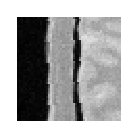
\includegraphics[width=2.5cm]{nn.eps}}\label{sfig:interpolation:nn}
\subfigure[]{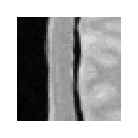
\includegraphics[width=2.5cm]{linear.eps}}\label{sfig:interpolation:lin}
\subfigure[]{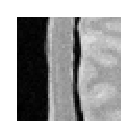
\includegraphics[width=2.5cm]{bs2.eps}}\label{sfig:interpolation:bs2}
\subfigure[]{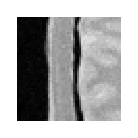
\includegraphics[width=2.5cm]{bs3.eps}}\label{sfig:interpolation:bs3}
\subfigure[]{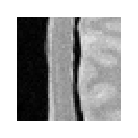
\includegraphics[width=2.5cm]{bs5.eps}}\label{sfig:interpolation:bs5}
\caption{Interpolation. (a) nearest neighbour, (b) linear, (c) B-spline $N=2$,
(d) B-spline $N=3$, (e) B-spline $N=5$.} \label{fig:interpolation}
\end{figure}

\section{Transforms}\label{sec:comp:transform}

The transformation model used for $\vT_{\vmu}$ determines what type of
deformations between the fixed and moving image you can handle. In order of
increasing flexibility, these are the translation, the rigid, the similarity,
the affine, the nonrigid B-spline and the nonrigid thin-plate spline like
transformations.

\begin{description}
\item[Translation:] (\texttt{TranslationTransform}) The translation is defined as:
\begin{align}
\vTmx &= \vx + \bm{t},
\end{align}
with $\bm{t}$ the translation vector. The parameter vector is
simply defined by $\vmu=\bm{t}$.

\item[Rigid:] (\texttt{EulerTransform}) A rigid transformation is defined as:
\begin{align}
\vTmx &= R (\vx - \bm{c}) + \bm{t} + \bm{c},
\end{align}
with the matrix $R$ a rotation matrix (i.e. orthonormal and
proper), $\bm{c}$ the centre of rotation, and $\bm{t}$ translation
again. The image is treated as a rigid body, which can translate
and rotate, but cannot be scaled/stretched. The rotation matrix is
parameterised by the Euler angles (one in 2D, three in 3D). The
parameter vector $\vmu$ consists of the Euler angles (in rad) and
the translation vector. In 2D, this gives a vector of length 3:
$\vmu = (\theta_z, t_x, t_y)^T$, where $\theta_z$ denotes the
rotation around the axis normal to the image. In 3D, this gives a
vector of length 6: $\vmu = (\theta_x, \theta_y, \theta_z, t_x,
t_y, t_z)^T$. The centre of rotation is not part of $\vmu$; it is
a fixed setting, usually the centre of the image.

\item[Similarity:] (\texttt{SimilarityTransform}) A similarity transformation is defined as
\begin{align}
\vTmx &= s \bm{R} (\vx - \bm{c}) + \bm{t} + \bm{c},
\end{align}
with $s$ a scalar and $\bm{R}$ a rotation matrix. This means that the image
is treated as an object, which can translate, rotate, and scale
isotropically. The rotation matrix is parameterised by an angle in 2D, and
by a so-called ``versor'' in 3D (Euler angles could have been used as
well). The parameter vector $\vmu$ consists of the angle/versor, the
translation vector, and the isotropic scaling factor. In 2D, this gives a
vector of length 4: $\vmu = (s, \theta_z, t_x, t_y)^T$. In 3D, this gives a
vector of length 7: $\vmu = (q_1, q_2, q_3, t_x, t_y, t_z, s)^T$, where
$q_1$, $q_2$, and $q_3$ are the elements of the versor. There are few cases
when you need this transform.

\item[Affine:] (\texttt{AffineTransform}) An affine transformation is defined as:
\begin{align}
\vTmx &= \bm{A} (\vx - \bm{c}) + \bm{t} + \bm{c},
\end{align}
where the matrix $\bm{A}$ has no restrictions. This means that the image
can be translated, rotated, scaled, and sheared. The parameter vector
$\vmu$ is formed by the matrix elements $a_{ij}$ and the translation
vector. In 2D, this gives a vector of length 6: $\vmu=(a_{11}, a_{12},
a_{21}, a_{22}, t_x, t_y)^T$. In 3D, this gives a vector of length 12.

\item[B-splines:] (\texttt{BSplineTransform}) For the category of non-rigid
    transformations, B-splines \citep{RueckertEA99} are often used as a
    parameterisation:
\begin{align}
\vTmx = \vx + \sum_{\vx_k \in \Ncal_{\vx}} \bm{p}_k \bm{\beta}^3(\vx
- \vx_k),\label{eq:bspline}
\end{align}
with $\vx_k$ the control points, $\bm{\beta}^3(x)$ the cubic
multidimensional B-spline polynomial \citep{Unser99}, $\bm{p}_k$ the
B-spline coefficient vectors (loosely speaking, the control point
displacements), and $\Ncal_{\vx}$ the set of all control points within the
compact support of the B-spline at $\vx$. The control points $\vx_k$ are
defined on a regular grid, overlayed on the fixed image. In this context we
talk about `the control point grid that is put on the fixed image', and
about `control points that are moved around'. Note that $\vTm(\vx_k)\neq
\vx_k + \bm{p}_k$, a common misunderstanding. Calling $\bm{p}_k$ the
control point displacements is, therefore, actually somewhat misleading.
Also note that the control point grid is entirely unrelated to the grid
used by the Grid image sampler, see Section~\ref{sec:comp:sampler}.

The control point grid is defined by the amount of space between the
control points, which can be different for each direction. B-splines
have local support ($|\Ncal_{\vx}|$ is small), which means that the
transformation of a point can be computed from only a couple of
surrounding control points. This is beneficial both for modelling
local transformations, and for fast computation. The parameters
$\vmu$ are formed by the B-spline coefficients $\bm{p}_k$. The
number of control points $P$ determines the number of parameters.
For 3D images, $\approx 10000$ parameters is not an unusual case.
The parameter vector is (for 2D images) composed as follows: $\vmu =
(p_{1x}, p_{2x}, \ldots, p_{Px}, p_{1y}, p_{2y}, \ldots, p_{Py}
)^T$.


\item[Thin-plate splines:] (\texttt{SplineKernelTransform}) Thin-plate
    splines are another well-known representation for nonrigid
    transformations. The thin-plate spline is an instance of the more
    general class of kernel-based transforms \cite{Davis97,Brooks07}. The
    transformation is based on a set of $k=1\ldots K$ corresponding
    landmarks in fixed and moving image. The landmark displacements
    $\bm{d}_k = \vx_k^{\mathrm{mov}} - \vx_k^{\mathrm{fix}}$ form the
    parameter vector $\vmu$. The fixed landmark positions
    $\vx_k^{\mathrm{fix}}$ are given by the user. The transformation is
    expressed as a sum of an affine component and a nonrigid component:
\begin{align}
\vTmx = \vx + A \vx + \bm{t} + \sum_{\vx_k} \bm{c}_k \bm{G}(\vx
- \vx_k^{\mathrm{fix}}),\label{eq:splinekernel}
\end{align}
 where $\vx_k$ are landmark positions in the fixed image, $\bm{G}(\bm{r})$
 is a basis function and $\bm{c}_k$ are the coefficients corresponding to
 each landmark. The coefficients $\bm{c}_k$ and the elements of $\bm{A}$
 and $\bm{t}$ are computed from the landmark displacements. The specific
 choice of basis function $\bm{G}(\bm{r})$ determines the ``physical
 behaviour''. The most often used choice of $\bm{G}(\bm{r})$ leads to the
 thin-plate spline, but another useful alternative is the elastic-body
 spline \cite{Davis97}. The spline kernel transforms are often less
 efficient than the B-splines (because they lack the compact support
 property of the B-splines), but they allow for more flexibility in placing
 the control points $\vx_k^{\mathrm{fix}})$. The parameter vector is (for
 2D images) composed as follows: $\vmu = (d_{1x}, d_{1y}, d_{2x}, d_{2y},
 \ldots, d_{Kx}, d_{Ky} )^T$. Note the difference in ordering of $\vmu$
 compared to the B-splines transform.
\end{description}

\begin{figure}
\centering
% was fixed.eps, moving.eps, deformed.eps
\subfigure[fixed]{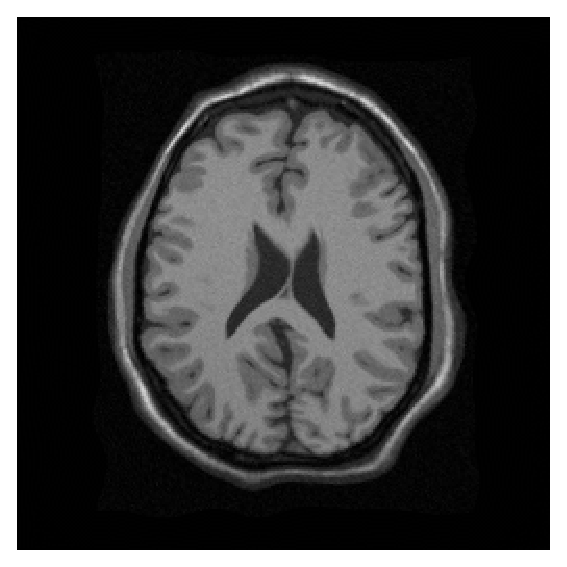
\includegraphics[width=4.5cm,height=4.5cm]{transformexample_fixed.eps}}\label{sfig:transformexample:a}
\subfigure[moving]{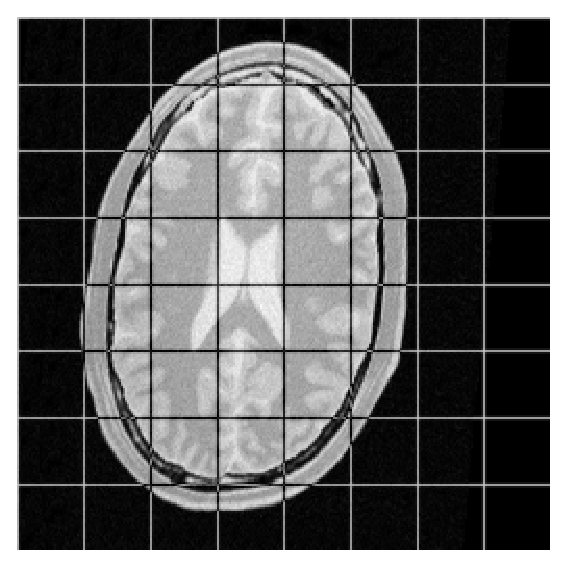
\includegraphics[width=4.5cm,height=4.5cm]{transformexample_orig.eps}}\label{sfig:transformexample:b}
\subfigure[translation]{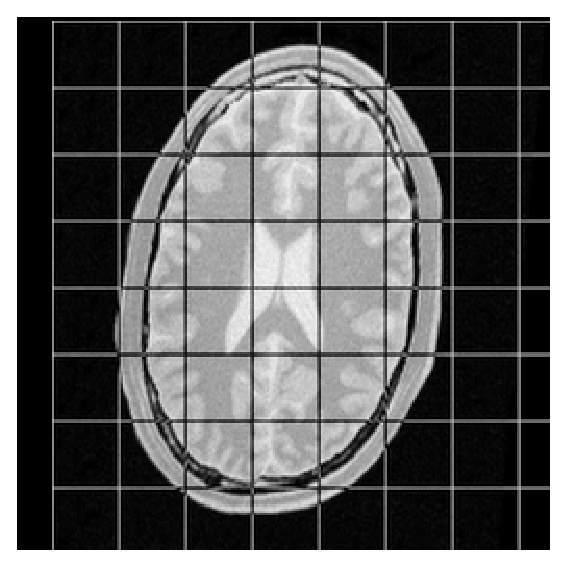
\includegraphics[width=4.5cm,height=4.5cm]{transformexample_tran.eps}}\label{sfig:transformexample:c}
\subfigure[rigid]{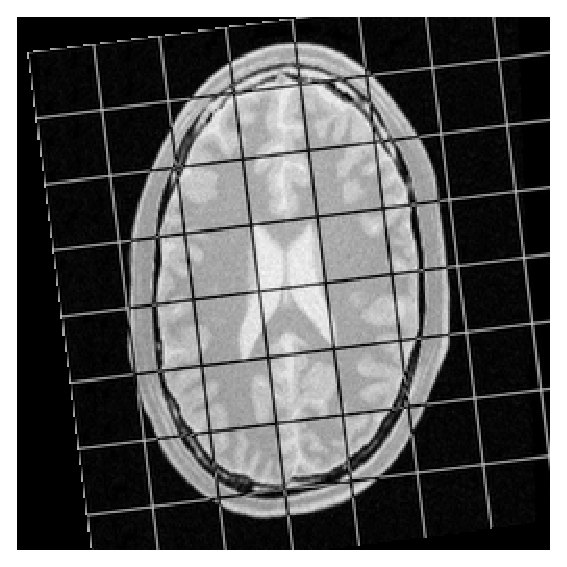
\includegraphics[width=4.5cm,height=4.5cm]{transformexample_rig.eps}}\label{sfig:transformexample:d}
\subfigure[affine]{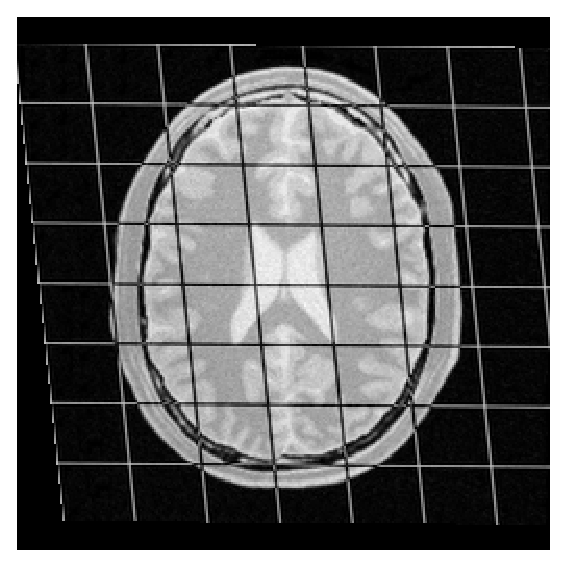
\includegraphics[width=4.5cm,height=4.5cm]{transformexample_aff.eps}}\label{sfig:transformexample:e}
\subfigure[B-spline]{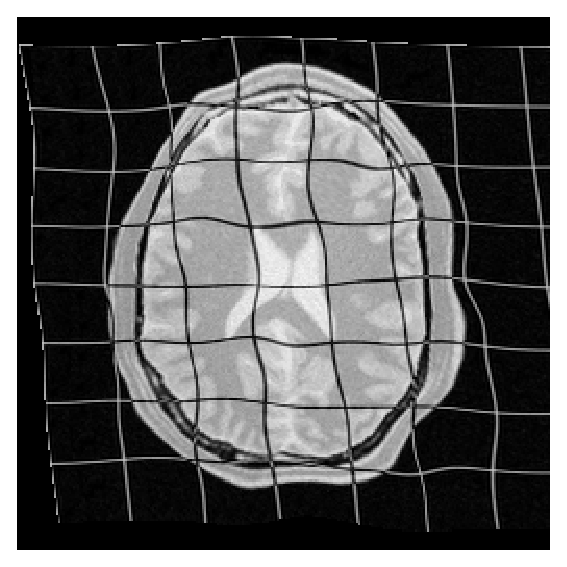
\includegraphics[width=4.5cm,height=4.5cm]{transformexample_bsp.eps}}\label{sfig:transformexample:f}
\caption{Different transformations. (a) the fixed image, (b) the
moving image with a grid overlayed, (c) the deformed moving image
$I_M(\vTmx)$ with a translation transformation, (d) a rigid
transformation, (e) an affine transformation, and (f) a B-spline
transformation. The deformed moving image nicely resembles the
fixed image $I_F(\vx)$ using the B-spline transformation. The
overlay grids give an indication of the deformations imposed on
the moving image. NB: the overlayed grid in (f) is NOT the
B-spline control point grid, since that one is defined on the
fixed image!} \label{fig:transformexample}
\end{figure}
See Figure \ref{fig:transformexample} for an illustration of different
transforms. Choose the transformation that fits your needs: only choose a
nonrigid transformation if you expect that the underlying problem contains
local deformations, choose a rigid transformation if you only need to
compensate for differences in pose. To initialise a nonrigid registration
problem, perform a rigid or affine one first. The result of the initial rigid
or affine registration $\vT_{\hat\vmu_0}$ is combined with a nonrigid
transformation $\vTm^\mathrm{NR}$ in one of the following two ways:
\begin{align}
  \text{addition: }\quad    & \vTmx = \vTm^\mathrm{NR}(\vx) + \vT_{\hat\vmu_0}(\vx) - \vx\label{eq:addition} \\
  \text{composition: }\quad & \vTmx = \vTm^\mathrm{NR}\left( \vT_{\hat\vmu_0}(\vx) \right)
  = ( \vTm^\mathrm{NR} \circ
  \vT_{\hat\vmu_0})(\vx)\label{eq:composition}
\end{align}
The latter method is in general to be preferred, because it makes
several postregistration analysis tasks somewhat more
straightforward.

%// iets over scales?

\section{Optimisers}\label{sec:comp:optimiser}

\begin{figure}
\centering
% was: Gradient_descent.eps
\includegraphics[width=0.8\textwidth]{gd_example.eps}
\caption{Iterative optimisation. Example for registration with a
translation transformation model. The arrows indicate the steps
$a_k \bm{d}_k$ taken in the direction of the optimum, which is the
minimum of the cost function.} \label{fig:optimisation}
\end{figure}
To solve the optimisation problem (\ref{eq:parametric}), i.e. to
obtain the optimal transformation parameter vector $\hat\vmu$,
commonly an iterative optimisation strategy is employed:
\begin{align}
\vmu_{k+1} &= \vmu_k + a_k \bm{d}_k, \quad k = 0, 1, 2, \cdots,
\end{align}
with $\bm{d}_k$ the `search direction' at iteration $k$, $a_k$ a
scalar gain factor controlling the step size along the search
direction. The optimisation process is illustrated in Figure
\ref{fig:optimisation}. \citet{KleinEA07} give an overview of
various optimisation routines the literature offers. Examples are
quasi-Newton (QN), nonlinear conjugate gradient (NCG), gradient
descent (GD), and Robbins-Monro (RM). Gradient descent and
Robbins-Monro are discussed below. For details on other
optimisation methods we refer to \citep{KleinEA07,NocedalEA99}.

\begin{description}
\item[Gradient descent (GD):] (\texttt{StandardGradientDescent}
or \texttt{RegularStepGradientDescent}) Gradient descent optimisation
methods take the search direction as the negative gradient of the
cost function:
\begin{align}
\vmu_{k+1} &= \vmu_k - a_k \bm{g}(\vmu_k),\label{eq:gd}
\end{align}
with $\bm{g}(\vmu_k) = \partial \mathcal{C} / \partial \vmu$
evaluated at the current position $\vmu_k$. Several choices exist for
the gain factor $a_k$. It can for example be determined by a line
search or by using a predefined function of $k$.

\item[Robbins-Monro (RM):]
(\texttt{StandardGradientDescent} or
\texttt{FiniteDifferenceGradientDescent}) The RM optimisation
method replaces the calculation of the derivative of the cost
function $\bm{g}(\vmu_k)$ by an approximation
$\widetilde{\bm{g}}_k$.
\begin{align}
\vmu_{k+1} &= \vmu_k - a_k \widetilde{\bm{g}}_k,\label{eq:RM}
\end{align}
The approximation is potentially faster to compute, but might
deteriorate convergence properties of the GD scheme, since every
iteration an approximation error $\bm{g}(\vmu_k) -
\widetilde{\bm{g}}_k$ is made. \citet{KleinEA07} showed that using
only a small random subset of voxels (\mbox{$\approx 2000$}) from
the fixed image accelerates registration significantly, without
compromising registration accuracy. The Random or RandomCoordinate
samplers, described in Section~\ref{sec:comp:sampler}, are
examples of samplers that pick voxels randomly. It is important
that a new subset of fixed image voxels is selected every
iteration $k$, so that the approximation error has zero mean. The
RM method is usually combined with $a_k$ as a predefined decaying
function of $k$:
\begin{align}
a_k &= \frac{a}{(k+A)^{\alpha}},\label{eq:gain}
\end{align}
where $a > 0$, $A \ge 1$, and $0 \le \alpha \le 1$ are
user-defined constants. In our experience, a reasonable choice is
$\alpha \approx 0.6$ and $A$ approximately 10\% of the
user-defined maximum number of iterations, or less. The choice of
the overall gain, $a$, depends on the expected ranges of $\vmu$
and $\bm{g}$ and is thus problem-specific. In our experience, the
registration result is not very sensitive to small perturbations
of these parameters. Section~\ref{sec:optimizertuning} gives some
more advice.
\end{description}

Note that GD and RM are in fact very similar. Running RM with a Full sampler
(see Section~\ref{sec:comp:sampler}), instead of a Random sampler, is
equivalent to performing GD. We recommend the use of RM over GD, since it is so
much faster, without compromising on accuracy. In that case, the parameter $a$
is the parameter that is to be tuned for your application. A more advanced
version of the \texttt{StandardGradientDescent} is the
\texttt{AdaptiveStochasticGradientDescent}, which requires less parameters to
be set and tends to be more robust \cite{Klein09}.

Other optimisers available in \elastix\ are: \texttt{FullSearch},
\texttt{ConjugateGradient}, \texttt{ConjugateGradientFRPR},
\texttt{QuasiNewtonLBFGS}, \texttt{RSGDEachParameterApart},
\texttt{SimultaneousPerturbation}, \texttt{CMAEvolutionStrategy}.

\section{Multi-resolution}\label{sec:comp:multiresolution}

For a good overview of multi-resolution strategies see
\citet{LesterEA99}. Two hierarchical methods are distinguished:
reduction of data complexity, and reduction of transformation
complexity.

\subsection{Data complexity}

It is common to start the registration process using images that have
lower complexity, e.g., images that are smoothed and possibly
downsampled. This increases the chance of successful registration. A
series of images with increasing amount of smoothing is called a
scale space. If the images are not only smoothed, but also
downsampled, the data is not only less complex, but the \emph{amount}
of data is actually reduced. In that case, we talk about a
``pyramid''. However, confusingly, the word pyramid is used by us
also to refer to a scale space. Several scale spaces or pyramids are
found in the literature, amongst others Gaussian and Laplacian
pyramids, morphological scale space, and spline and wavelet pyramids.
The Gaussian pyramid is the most common one. In \elastix\ we have:
\begin{description}
\item[Gaussian pyramid:] (\texttt{FixedRecursiveImagePyramid} and
\texttt{MovingRecursiveImagePyramid}) Applies smoothing and
down-sampling.

\item[Gaussian scale space:] (\texttt{FixedSmoothingImagePyramid} and
\texttt{MovingSmoothingImagePyramid}) Applies smoothing and
\emph{no} down-sampling.

\item[Shrinking pyramid:] (\texttt{FixedShrinkingImagePyramid} and
\texttt{MovingShrinkingImagePyramid}) Applies \emph{no} smoothing,
but only down-sampling.
\end{description}

Figure~\ref{fig:multiresolution} shows the Gaussian pyramid with and
without downsampling. In combination with a Full sampler (see
Section~\ref{sec:comp:sampler}), using a pyramid with downsampling
will save a lot of time in the first resolution levels, because the
image contains much fewer voxels. In combination with a Random
sampler, or RandomCoordinate, the downsampling step is not necessary,
since the random samplers select a user-defined number of samples
anyway, independent of the image size.

\begin{figure}
\centering
\subfigure[resolution 0]{
\includegraphics[width=3cm]{moving_pd.R0d.eps}}
\subfigure[resolution 1]{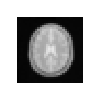
\includegraphics[width=3cm]{moving_pd.R1d.eps}}
\subfigure[resolution 2]{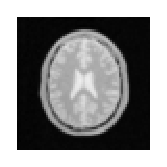
\includegraphics[width=3cm]{moving_pd.R2d.eps}}
\subfigure[original]{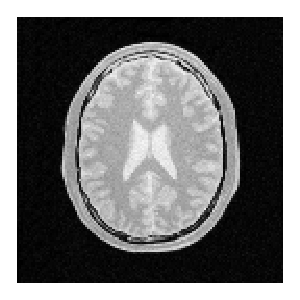
\includegraphics[width=3cm]{moving_pd.128.eps}} \\
\subfigure[resolution
0]{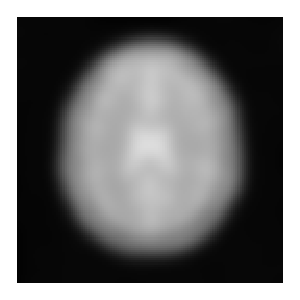
\includegraphics[width=3cm]{moving_pd.R0.eps}}
\subfigure[resolution
1]{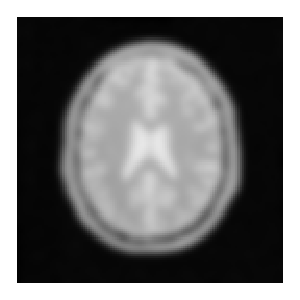
\includegraphics[width=3cm]{moving_pd.R1.eps}}
\subfigure[resolution
2]{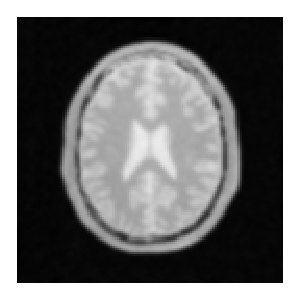
\includegraphics[width=3cm]{moving_pd.R2.eps}}
\subfigure[original]{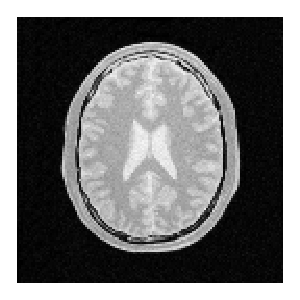
\includegraphics[width=3cm]{moving_pd.128.eps}}
\caption{Two multi-resolution strategies using a Gaussian pyramid
($\sigma = 8.0, 4.0, 2.0$ voxels). The first row shows
multi-resolution with down-sampling
(\texttt{FixedRecursiveImagePyramid}), the second row without
(\texttt{FixedSmoothingImagePyramid}). Note that in the first row,
for each dimension, the image size is halved every resolution, but
that the voxel size increases with a factor 2, so physically the
images are of the same size every resolution.}
\label{fig:multiresolution}
\end{figure}

\subsection{Transformation complexity}

The second multiresolution strategy is to start the registration
with fewer degrees of freedom for the transformation model. The
degrees of freedom of the transformation equals the length (number
of elements) of the parameter vector $\vmu$.

An example of this was already mentioned in Section~\ref{sec:comp:transform}:
the use of a rigid transformation prior to nonrigid (B-spline) registration. We
may even use a three-level strategy: first rigid, then affine, then nonrigid
B-spline.

Another example is to increase the number of degrees of freedom
within the transformation model. With a B-spline transformation,
it is often good practice to start registration with a coarse
control point grid, only capable of modelling coarse deformations.
In subsequent resolutions the B-spline grid is gradually refined,
thereby introducing the capability to match smaller structures.
See Section~\ref{sec:transformtuning}.

\section{Evaluating registration}\label{sec:evaluation}

How do you verify that your registration was successful? This is a
difficult problem. In general, you don't know for each voxel where
it should map to. Here are some hints:

\begin{itemize}
\item The deformed moving image $I_M(\vT_{\vmu}(\vx))$ should
look similar to the fixed image $I_F(\vx)$. So, compare images side
by side in a viewer. You can also display the two images on top of
each other with a checkerboard view or a dragable cross. Besides
looking similar, also check that the deformed moving image has the
same texture as the moving image. Sudden blurred areas in the
deformed image may indicate that the deformation at that region is
too large.

\item For mono-modal image data you can inspect the difference
image. Perfect registration would result in a difference image
without any edges, just noise.

\item Compute the overlap of segmented anatomical structures
after registration. The better the overlap, the better the
registration. To measure overlap, commonly the Dice similarity
coefficient (DSC) is used:
\begin{equation}
  \mathrm{DSC}(X,Y) = \frac{2 |X \cap Y|}{|X|+|Y|},
\end{equation}
where $X$ and $Y$ represent the binary label images, and $|\cdot|$
denotes the number of voxels that equal 1. A higher DSC indicates a
better correspondence. A value of 1 indicates perfect overlap, a
value of 0 means no overlap at all. Also the Tannimoto (TC)
coefficient is used often. It is related to the DSC by
$\mathrm{DSC}=2\mathrm{TC}/(\mathrm{TC}+1)$. See also
\cite{Cru06:Generalized}. It is important to realise that the
surface-volume ratio of the segmented structures influences the
overlap values you typically get \citep{Roh04:Evaluation}. A value
of $\mathrm{DSC}=0.8$ would be very good for the overlap of complex
vessel structures. For large spherical objects though, an overlap
$<0.9$ is in general not very good. What is good enough depends of
course on your application.

\item Compute the distance after registration between points that you know correspond.
You can obtain corresponding points by manually clicking them in the
fixed and the moving image. A less time-consuming option is the
semi-automated approach of Murphy \etal\ \cite{Murphy08}, which is
designed for finding corresponding points in the lung. Ideally, the
registration has found the same correspondence as the ground truth.

\item Inspect the deformation field by looking at the determinant of
the Jacobian of $\vTmx$. Values smaller than 1 indicate local
compression, values larger than 1 indicate local expansion, and 1
means volume preservation. If this value deviates substantially
from 1, you may be worried (but maybe not if this is what you
expect for your application). In case it is negative you have
``foldings'' in your transformation, and you definitely should be
worried.

\item Inspect the convergence, by computing for each iteration
the exact metric value (and not an approximated value, when you do
random sampling), and plot it. For example for the SSD measure,
the lower the metric value, the better the registration.

\end{itemize}

% There are papers about evaluation of registration


%%%%%%%%%%%%%%%%%%%%%%%%%%%%%%%%%%%%%%%%%%%%%%%%%%%%%%%%%%%%%%%%%%%%%%%%%%%%%%%%%%%%%%%%%%%%

\chapter{\elastix}\label{chp:elastix}

\section{Introduction}\label{sec:elastix:intro}

The development of \elastix\ started half to late 2003, and was intended to
facilitate our registration research. After some initial versions we decided to
put the separate components of \elastix\ in separate libraries. This resulted
in major version 3.0 in November 2004. \elastix\ 3.0 was also the first version
that was made publicly available on the \elastix\ website, around the same
time. The continued development brings us today (\today) to version 4.3.

\begin{table}[h!]
\begin{tabular}{l|l}
what & where \\
\hline
website        & \url{http://elastix.isi.uu.nl} \\
SVN repository & \url{https://svn.bigr.nl/elastix/trunkpublic} \\
WIKI           & \url{http://elastix.isi.uu.nl/wiki.php} \\
FAQ            & \url{http://elastix.isi.uu.nl/FAQ.php} \\
Mailing list   & \url{elastix@bigr.nl} (subscription via website) \\
\end{tabular}
\end{table}

The website also contains a
\texttt{doxygen}\footnote{\url{http://www.doxygen.org}} generated part that
provides documentation of the source code. An overview of all available classes
can be found at
\begin{quote}
\url{http://elastix.isi.uu.nl/doxygen/classes.html}.
\end{quote}
For each class a description of this class is given, together with
information on how to use it in \elastix. See
\begin{quote}
\url{http://elastix.isi.uu.nl/doxygen/modules.html}
\end{quote}
for an overview of all available components.

\subsection{Key features}\label{sec:elastix:key}

\elastix\ is
\begin{itemize}
\item open source, freely available from \url{http://elastix.isi.uu.nl};

\item based on the ITK, so the code base is thoroughly tested.
Quite some modifications/additions are made to the original ITK
code though, such as the use of samplers, a transformation class
that combines multiple transformation using composition or
addition, and more.

\item suitable for many image formats. The use of ITK implies that
all image formats supported by ITK are supported by \elastix. Some
often used (medical) image formats are: .mhd (MetaIO), .hdr
(Analyze/NIfTI), .gipl, .dcm (DICOM slices). DICOM directories are
not directly supported by \elastix;

\item multi-platform (at least Windows, Linux and Mac OS), multi-compiler
(at least Visual C++ 2005, 2008, gcc 3.2, 4.02, 4.1.2), and supports
32 and 64 bit systems. The underlying ITK code builds on many more
platforms, see \url{www.itk.org/Wiki/ITK_Prerequisites}. So, it is
highly portable to the platform of the user's choice;

\item highly configurable: there is a lot of choice for all the registration
components. Choosing the configuration that suits your needs is easy
thanks to human readable and editable parameter file;

\item easy to use for large amounts of data, since \elastix\ can be
called easily in a script;

\item fast, thanks to stochastic subsampling, if desired;

\item relatively easy to extend, i.e. to add new components, so it is
very suited for research also.
\end{itemize}

\section{Getting started}\label{sec:elastix:install}

This section describes how you can install \elastix, either directly
from the binaries, or by compiling \elastix\ yourself.

\subsection{Getting started the really easy way}

The easiest way to get started with \elastix\ is to use the
pre-compiled binaries.
\begin{enumerate}
\item Download the compressed archive from the website:
    \begin{quote}
    \url{http://elastix.isi.uu.nl/download.php}
    \end{quote}

\item Extract the archive to a \texttt{folder} of your choice.

\item Make sure your operating system can find the program:
    \begin{enumerate}
    \item Windows XP: Go to the control panel, go to ``System'', go to
    the tab ``Advanced'', click ``Environmental variables'', add \texttt{folder}
    to the variable ``path''.

    \item Linux: Add \texttt{folder} to the path by adding the line
    ``\texttt{export PATH=folder:\$PATH}'' to your \texttt{.bashrc} file.
    \end{enumerate}
    or call \elastix\ with the full path:
    \texttt{fullPathToFolder$\backslash$folder$\backslash$elastix}
\end{enumerate}

\subsection{Getting started the easy way}

It is also possible to compile \elastix\ yourself, since the source code is
freely available. In this section, we assume you use the Microsoft Visual C++
2003 (or higher) compiler under Windows, and the GCC compiler under Linux.

\begin{enumerate}
\item Download and install CMake: \url{www.cmake.org}.

\item Download and compile the ITK version 3.20: \url{www.itk.org}.
Make sure to set the following (advanced) CMake variables to
\texttt{ON}: \texttt{ITK\_USE\_REVIEW},
\texttt{ITK\_USE\_REVIEW\_STATISTICS},
\texttt{ITK\_USE\_ORIENTED\_IMAGE\_DIRECTION},
\texttt{ITK\_IMAGE\_BEHAVES\_AS\_ORIENTED\_IMAGE},
\texttt{ITK\_USE\_CENTERED\_PIXEL\_COORDINATES\_CONSISTENTLY}. On
Linux systems with the GCC compiler: set \texttt{CMAKE\_BUILD\_TYPE}
to ``Release''.

%1. Download cmake from www.cmake.org and install it according to instructions
%2. Download itk 3.12 from www.itk.org (not version 3.10).
%3. Unpack the ITK tarball
%4. make a directory where you want to generate the binaries and go that directory
%5. run: ccmake <ITKsourcedir>
%    In the Cmake interface you have to repeatedly press c (configure) until the "generate" option becomes available.
%    Also you have to make some choices:
%    BuildType = Release
%    BuildExamples / BuildTesting / BuildSharedLibs = Off
%    At the end, press generate (g)
%7. download the elastix sources and unpack
%8. follow the same procedure as with itk: generate a directory for the binaries, go to there, and run: ccmake <elastixsourcedir>
%9. BuildType= Release
%    ITK_DIR = the binary directory where you compiled itk
%    CMAKE_INSTALL_PREFIX = choose a directory where you would like to install the elastix executables
%10. run: make install

\item Download the compressed sources from the website.

\item Extract the archive to a \texttt{folderSrc} of your choice.

\item Run CMake on \elastix:
    \begin{enumerate}
    \item Windows: start CMake. Find the \texttt{folderSrc} with the
    source code. Set the folder where you want the binaries to be
    created. Click ``Configure'' and select the compiler that you
    use. Set the \texttt{CMAKE\_INSTALL\_PREFIX} to the directory
    where you want \elastix\ installed. Click ``Configure'' until
    all cache values are no longer red, and click OK.

    \item Linux: run CMake from the folder where you want the
    binaries to be created, with as command line argument the folder
    in which the sources were extracted: \texttt{ccmake folderSrc}.
    Set the \texttt{CMAKE\_BUILD\_TYPE} to ``Release'' and the
    \texttt{CMAKE\_INSTALL\_PREFIX} to the directory where you want
    \elastix\ installed.
    \end{enumerate}
CMake will create a project or solution or make file for your
compiler.

\item Compile \elastix\ by opening the project and selecting ``compile'' in
    release mode, or on Linux by running \texttt{make install}. Your
    compiler will now create the \elastix\ binaries.

\item Make sure your operating system can find the program, see
above.
\end{enumerate}

For developers: When running CMake, you may toggle the display of
the ``advanced'' options. In this list you will find several
options like \texttt{USE\_BSplineTransform ON/OFF}. By default all
are ON. To reduce compilation time, you may turn some components
OFF, which you do not plan to use anyway. Be careful though to not
turn off essential components.

\section{How to call \elastix}\label{sec:elastix:call}

\elastix\ is a command line program. This means that you have to
open a command line interface (a DOS-box, a shell) and type in an
appropriate \elastix\ command. This also means that there is no
graphical user interface. Help on using the program can be acquired
as follows:
\begin{quote}
\texttt{elastix --help}
\end{quote}
which will give a list of mandatory and optional arguments. The most
basic command to run a registration is as follows:
\begin{quote}
\texttt{elastix -f fixedImage.ext -m movingImage.ext -out
outputDirectory -p parameterFile.txt}
\end{quote}
where `\texttt{ext}' is the extension of the image files. The above
arguments are mandatory. These are minimally needed to run \elastix.
The parameter file is an important file: it contains, in normal
text, what kind of registration is performed (i.e. what metric,
optimiser, etc.) and what the parameters are that define the
registration. It gives a high amount of flexibility and control over
the process. More information about the parameter file is given in
Section \ref{sec:elastix:param}. All output of \elastix\ is written
to the output directory, which needs to be created before running
\elastix. The output consists of a log file (\texttt{elastix.log}),
the parameters of the transformation $\vT_{\vmu}$ that relates the
fixed and the moving image (\texttt{TransformParameters.?.txt}),
and, optionally, the resulting registered image $I_M(\vTmx)$
(\texttt{result.?.mhd}). The log file contains all messages that
were print to screen during registration. Also the
\texttt{parameterFile.txt} is copied into the log file, and the
contents of the \texttt{TransformParameters.?.txt} files are
included. The log file is thus especially useful for trouble
shooting.

Besides the mandatory arguments, there are some optional
arguments. Mask images can be provided by adding \texttt{-fMask
fixedMask.ext} and/or \texttt{-mMask movingMask.ext} to the
command line. An initial transformation can be provided with a
valid transform parameter file by adding \texttt{-t0
TransformParameters.txt} to the command line. With the command
line option \texttt{-threads unsigned\_int} the user can specify
the maximum number of threads that \elastix\ will use.

Running multiple registrations in succession, each possibly of a
different type, and with the output of a previous registration as
input to the next, can be done with \elastix\ in several ways. The
first one is to run \elastix\ once with the first registration, and
use its output (the \texttt{TransformParameter.0.txt} that can be
found in the output directory) as input for a new run of \elastix\
with the command line argument \texttt{-t0}. So:
\begin{quote}
\texttt{elastix -f ... -m ... -out out1 -p param1.txt} \\
\texttt{elastix -f ... -m ... -out out2 -p param2.txt -t0
out1/TransformParameters.0.txt} \\
\texttt{elastix -f ... -m ... -out out3 -p param3.txt -t0
out2/TransformParameters.0.txt}
\end{quote}
and so on. Another possibility is combine the registrations with one
run of \elastix:
\begin{quote}
\texttt{elastix ... -p param1.txt -p param2.txt -p param3.txt}
\end{quote}
The transformations from each of the registrations are automatically
combined, using one of the equations (\ref{eq:addition}) and
(\ref{eq:composition}).

On the \elastix-website, in the `About' section, you can find an
example on how to use the program. Maybe now is the time to try
the example and see a registration in action.


\section{The parameter file}\label{sec:elastix:param}

The parameter file is a text file that defines the components of the
registration and their parameter values. Supplying a parameter works
as follows:
\begin{quote}
\texttt{(ParameterName value(s))}
\end{quote}
So parameters are provided between brackets, first the name,
followed by one or more values. If the value is of type string then
the values need to be quoted:
\begin{quote}
\texttt{(ParameterName "value1" ... "valueN")}
\end{quote}
Comments can be provided by starting the line with `\texttt{//}'. A
minimal example of a valid parameter file is given in Appendix
\ref{chp:ExampleParam}. A list of available parameters for each
class is given at
\url{http://elastix.isi.uu.nl/doxygen/parameter.html}. Examples of
parameter files can be found at the wiki:
\url{http://elastix.bigr.nl/wiki/index.php/Parameter_file_database}.

Since the choice of the several components and the parameter values
define the registration, it is very important to set them wisely.
These choices are what make the registration a success or a disaster.
Therefore, a separate chapter is dedicated to the fine art of tuning
a registration, see Chapter \ref{chp:Tutorial}.


%%%%%%%%%%%%%%%%%%%%%%%%%%%%%%%%%%%%%%%%%%%%%%%%%%%%%%%%%%%%%%%%%%%%%%%%%%%%%%%%%%%%%%%%%%%%

\chapter{\transformix}\label{chp:transformix}

\section{Introduction}

By now you are able to at least run a registration, by calling
\elastix\ correctly. It is often also useful to apply the
transformation as found by the registration to another image.
Maybe you want to apply the transformation to an original (larger)
image to gain resolution. Or maybe you need the transformation to
apply it to a label image (segmentation). For those purposes a
program called \transformix\ is available. It was developed
simultaneously with \elastix.

\section{How to call \transformix}\label{sec:calltransformix}

Like \elastix, \transformix\ is a command line driven program. You
can get basic help on how to call it, by:
\begin{quote}
\texttt{transformix --help}
\end{quote}
which will give a list of mandatory and optional arguments.

The most basic command is as follows:
\begin{quote}
\texttt{transformix -in inputImage.ext -out outputDirectory -tp
TransformParameters.txt}
\end{quote}
This call will transform the input image and write it, together
with a log file \texttt{transformix.log}, to the output directory.
The transformation you want to apply is defined in the transform
parameter file. The transform parameter file could be the result
of a previous run of \elastix\ (see Section
\ref{sec:elastix:call}), but may also be written by yourself.
Section~\ref{sec:transformix:tp} explains the structure and
contents that a transform parameter file should have.

Besides using \transformix\ for deforming images, you can also use
\transformix\ to evaluate the transformation $\vTmx$ at some
points $\vx$. If you want to deform a set of user-specified
points, the appropriate call is:
\begin{quote}
\texttt{transformix -def inputPoints.txt -out outputDirectory -tp
TransformParameters.txt}
\end{quote}
This will create a file \texttt{outputpoints.txt} containing the
input points $\vx$ and the transformed points $\vTmx$ (both given
as voxel indices of the fixed image and as physical coordinates),
the displacement vector $\vTmx-\vx$ (in physical coordinates),
and, if \texttt{-in inputImage.ext} is also specified, the
transformed output points as indices of the input
image\footnote{The downside of this is that the input image is
also deformed, which consumes time and may not be needed by the
user. If this is a problem, just run \transformix\ without
\texttt{-in} and compute the voxel indices yourself, based on the
$\vTmx$ physical coordinate data.}. The \texttt{inputPoints.txt}
file should have the following structure:
\begin{quote}
\texttt{<index, point>}\\
\texttt{<number of points>}\\
\texttt{point1\_x point1\_y [point1\_z]}\\
\texttt{point2\_x point2\_y [point2\_z]}\\
\texttt{$\ldots$}
\end{quote}
The first line indicates whether the points are given as
``indices'' (of the fixed image), or as ``points'' (in physical
coordinates). The second line stores the number of points that
will be specified. After that the point data is given.

If you want to know the deformation at all voxels of the fixed
image, simply use \texttt{-def all}:
\begin{quote}
\texttt{transformix -def all -out outputDirectory -tp
TransformParameters.txt}
\end{quote}
The deformation field is stored as a vector image
\texttt{deformationField.mhd}. Each voxel contains the
displacement vector $\vTmx-\vx$ in physical coordinates. The
elements of the vectors are stored as \texttt{float} values.

In addition to computing the deformation field, \transformix\ has
the capability to compute the spatial Jacobian of the
transformation. The determinant of the spatial Jacobian identifies
the amount of local compression or expansion and can be quite
useful, for example in lung ventilation studies. The determinant of
the spatial Jacobian can be computed on the entire image only using:
\begin{quote}
\texttt{transformix -jac all -out outputDirectory -tp
TransformParameters.txt}
\end{quote}
The complete spatial Jacobian matrix can also be computed:
\begin{quote}
\texttt{transformix -jacmat all -out outputDirectory -tp
TransformParameters.txt}
\end{quote}
where each voxel is filled with a $d \times d$ matrix, with $d$ the
image dimension, instead of a simply a scalar value.

With the command-line option \texttt{-threads unsigned\_int} the
user can specify the maximum number of threads that \transformix\
will use.

\section{The transform parameter file}\label{sec:transformix:tp}

The result of a registration is the transformation $\vTm$ relating
the fixed and moving image. The parameters of this transformation
are stored in a \texttt{TransformParameters.?.txt}-file. An
example of its structure for a 2D rigid transformation is given in
Appendix \ref{chp:ExampleTransformParam}. The text file contains
all information necessary to resample an input image (the moving
image) to the region specified in the file (by default the fixed
image region).

The transform parameter file can be manually edited or created as
is convenient for the user. Multiple transformations are composed
by iteratively supplying another transform parameter file with the
\texttt{InitialTransformParametersFileName} tag. The last
transformation will be the one where the initial transform
parameter file name is set to \texttt{"NoInitialTransform"}.

An important parameter in the transform parameter files is the
\texttt{FinalBSplineInterpolationOrder}. Usually it is set to 3, because that
produces the best quality result image after registration, see
Sec~\ref{sec:interpolatortuning}. However, if you use \transformix\ to deform a
\emph{segmentation} of the moving image (so, a binary image), you need to
manually change the \texttt{FinalBSplineInterpolationOrder} to 0. This will
make sure that the deformed segmentation is still a binary label image. If
third order interpolation is used, the deformed segmentation image will contain
garbage. This is related to the ``overshoot-property'' of higher-order B-spline
interpolation.

\section{Some details}

\subsection{Run-time}

The run-time of \transformix\ is built up of the following parts:

\begin{enumerate}
\item Computing the B-spline decomposition of the input image (in case you selected the
\texttt{FinalBSplineInterpolator});

\item Computing the transformation for each voxel;

\item Interpolating the input image for each voxel.
\end{enumerate}
We have never performed tests to measure the computational
complexity of each step, but we think that step 1 is the least
time-consuming task. This step can obviously be avoided by using a
nearest neighbour or linear interpolator. Step 2 is dependent on the
choice of the transformation, where linear transformations, such as
the rigid and affine transform, are substantially faster than
nonlinear transforms, such as the B-spline transform. Step 3 depends
on the specific interpolator. In order of increasing complexity:
nearest neighbour, linear, 1st-order B-spline, 2nd-order B-spline,
etc.

%[What is the complexity of FinalBSplineInterpolator? And of
%FinalLinearInterpolator? In required operations per voxel. Is that
%described in the docs, in some papers, or on the wiki?]

\subsection{Memory consumption}

For more information about memory consumption, see Section
\ref{ssec:tut:memory} and also:
\begin{quote}
\url{http://elastix.bigr.nl/wiki/index.php/Memory_consumption_transformix}
\end{quote}

%%%%%%%%%%%%%%%%%%%%%%%%%%%%%%%%%%%%%%%%%%%%%%%%%%%%%%%%%%%%%%%%%%%%%%%%%%%%%%%%%%%%%%%%%%%%

\chapter{Tutorial}\label{chp:Tutorial}


\section{Selecting the registration components}

When performing registration one carefully has to choose the
several components, as specified in Chapter
\ref{chp:Registration}. The components must be specified in the
parameter file. For example:
\begin{quote}
\texttt{(Transform "BSplineTransform")}\\
\texttt{(Metric "AdvancedMattesMutualInformation")}\\
$\ldots$
\end{quote}

In Table \ref{table:tutorial:components} a list of the components
that need to be specified is given, with some recommendations. The
``Registration'' component was not mentioned in
Chapter~\ref{chp:Registration}. The registration component serves
to connect all other components and implements the multiresolution
aspect of registration. So, one may say that it actually
implements the block scheme of
Figure~\ref{fig:registrationcomponents}. Also the ``Resampler''
component was not explicitly mentioned in
Chapter~\ref{chp:Registration}. It simply serves to generate the
deformed moving image after registration. Currently there is only
one Resampler available in \elastix: the
\texttt{DefaultResampler}. The component is therefore not further
discussed.

\begin{table}[htb]
\centering
\begin{tabular}{l|p{15em}}
\textbf{Component} & \textbf{Recommendation} \\
\hline
Registration & \texttt{MultiResolutionRegistration} \\
Metric       & \texttt{AdvancedMattesMutualInformation} \\
Sampler      & \texttt{RandomCoordinate} \\
Interpolator & \texttt{BSplineInterpolator} \\
ResampleInterpolator & \texttt{FinalBSplineInterpolator} \\
Resampler    & \texttt{DefaultResampler}\\
Transform    & Depends on the application \\
Optimizer    & \texttt{StandardGradientDescent}/ \texttt{AdaptiveStochasticGradientDescent} \\
FixedImagePyramid   & \texttt{FixedSmoothingImagePyramid} \\
MovingImagePyramid  & \texttt{MovingSmoothingImagePyramid} \\
\end{tabular}
\caption{Some recommendations for the several components.}\label{table:tutorial:components}
\end{table}

\section{Overview of all parameters}

A list of all available components of \elastix\ can be found at:
\begin{quote}
\url{http://elastix.isi.uu.nl/doxygen/modules.html}
\end{quote}
A list of all parameters that can be specified for each registration
component can be found at the \elastix\ website:
\begin{quote}
\url{http://elastix.isi.uu.nl/doxygen/parameter.html}
\end{quote}
At that site you can find how to specify a parameter and what the
default value is. We have tried to come up with sensible defaults,
although the defaults will certainly not work in all cases. A
collection of successful parameter files can be found at the wiki:
\begin{quote}
\url{http://elastix.bigr.nl/wiki/index.php/Parameter_file_database}
\end{quote}
This may get you started with your particular application.

\section{Important parameters}\label{sec:Tutorial:importantparam}

In the same order as in Section \ref{sec:comp:metric} we discuss
the important parameters for each component and explain the
recommendations made in Table~\ref{table:tutorial:components}.

\subsection{Registration}\label{sec:registrationtuning}

Just use the \texttt{MultiResolutionRegistration} method, since
multi-resolution is a good idea. And if you still think you don't
need all this multi-resolution, you can always set the
\texttt{NumberOfResolutions} to 1. You don't have to set anything
else. Section~\ref{sec:pyramidtuning} discusses the number of
resolutions in more detail.

\subsection{Metric}

The \texttt{AdvancedMattesMutualInformation} usually works well,
both for mono- and multi-modal images. It supports fast computation
of the metric value and derivative in case the transform is a
B-spline by exploiting its compact support. You need to set the
number of histogram bins, which is needed to compute the joint
histogram. A good value for this depends on the dynamic range of
your input images, but in our experience 32 is usually ok:
\begin{quote}
\texttt{(NumberOfHistogramBins 32)}
\end{quote}

\subsection{Sampler}\label{sec:samplertuning}

The \texttt{RandomCoordinate} sampler works well in conjunction with
the \texttt{StandardGradientDescent} and\\
\texttt{AdaptiveStochasticGradientDescent} optimisers, which are the
recommended optimisation routines. These optimisation methods can be
used with a small amount of samples, randomly selected in every
iteration, see Section \ref{sec:comp:optimiser}, which significantly
decreases registration time. Set the \texttt{NumberOfSpatialSamples}
to 3000. Don't go lower than 2000. Compared to samplers that draw
samples on the voxel-grid (such as the \texttt{Random} sampler), the
\texttt{RandomCoordinate} sampler avoids what is known as the
grid-effect \citep{The08:Halton}.

An important option for the random samplers, discussed in
Section~\ref{sec:optimizertuning} is:
\begin{quote}
  \texttt{(NewSamplesEveryIteration "true")}
\end{quote}
which enforces the selection of new samples in every iteration.

An interesting option for the \texttt{RandomCoordinate} sampler is
the \texttt{UseRandomSampleRegion} parameter, used in combination
with the \texttt{SampleRegionSize} parameter. If
\texttt{UseRandomSampleRegion} is set to \texttt{"false"} (the
default), the sampler draws samples from the entire image domain.
When set to \texttt{"true"}, the sampler randomly selects one
voxel, and then selects the remaining samples in a square
neighbourhood around that voxel. The size of the neighbourhood is
determined by the \texttt{SampleRegionSize} (in physical
coordinates). An example for 3D images:
\begin{quote}
  \texttt{(ImageSampler "RandomCoordinate")}\\
  \texttt{(NewSamplesEveryIteration "true")}\\
  \texttt{(UseRandomSampleRegion "true")}\\
  \texttt{(SampleRegionSize 50.0 50.0 50.0)}\\
  \texttt{(NumberOfSpatialSamples 2000)}\\
\end{quote}
In every iteration, a square region of $50^3$\,mm is randomly
selected. In that region, 2000 samples are selected according to a
uniform distribution. Effectively, a kind of \emph{localized}
similarity measure is obtained, which sometimes gives better
registration results. See \cite{Kle08:Automatic} for more
information on this approach. For the sample region size a
reasonable value to try is $\approx1/3$ of the image size.

\subsection{Interpolator}\label{sec:interpolatortuning}

During the registration, use the \texttt{BSplineInterpolator} with
first order interpolation:
\begin{quote}
\texttt{(BSplineInterpolationOrder 1)}
\end{quote}
We recommend this instead of the \texttt{LinearInterpolator},
since the \texttt{BSplineInterpolator} has a dedicated function to
compute the derivative of the moving image.

We recommend a higher quality third order B-spline interpolator for
generating the resulting deformed moving image:
\begin{quote}
\texttt{(ResampleInterpolator "FinalBSplineInterpolator")} \\
\texttt{(FinalBSplineInterpolationOrder 3)}
\end{quote}

\subsection{Transform}\label{sec:transformtuning}

This choice depends on the application at hand. For images of the
same patient where you expect no nonrigid deformation, you can
consider a rigid transformation, i.e. choose the
\texttt{EulerTransform}. If you want to compensate for differences
in scale, consider the affine transformation:
\texttt{AffineTransform}. These two transformations require a centre
of rotation, which can be set by the user. By default the geometric
centre of the fixed image is taken, which is recommended. Another
parameter that needs to be set is the \texttt{Scales}. The scales
define for each element of the transformation parameters $\vmu$ a
scaling value, which is used during optimisation. The scaling serves
to bring the elements of $\vmu$ in the same range (parameters
corresponding to rotation have in general a much smaller range than
parameters corresponding to translation). We recommend to let
\elastix\ compute it automatically:
\texttt{(AutomaticScalesEstimation "true")}\footnote{The
implementation is given in
%\verb=elastix\src\Core\ComponentBaseClasses\elxTransformBase.hxx=}
\texttt{elastix$\backslash$src$\backslash$Core$\backslash$ComponentBaseClasses$\backslash$elxTransformBase.hxx}}.
Always start with a rigid or affine transformation before doing a
nonrigid one, to get a good initial alignment.

For nonrigid registration problems \elastix\ has the
\texttt{BSplineTransform}. The B-spline nonrigid transformation is
defined by a uniform grid of control points. This grid is defined
by the spacing between the grid nodes. The spacing defines how
dense the grid is, or what the locality is of the transformation
you can model. For each resolution level you can define a
different grid spacing. This is what we call multi-grid. In
general, we recommend to start with a coarse B-spline grid, i.e. a
more global transformation. This way the larger structures are
matched first, for the same reason as why you should start with a
rigid or affine transformation. In later resolutions you can
refine the transformation in a stepwise fashion; the idea is that
you subsequently match smaller structures, up to the final
precision. The final grid spacing is specified with:
\begin{quote}
\texttt{(FinalGridSpacingInPhysicalUnits 10.0 10.0 10.0)}
\end{quote}
with as much numbers as there are dimensions in your image. The
spacing is in most medical images specified in millimetres. It is
also possible to specify the grid in voxel units:
\begin{quote}
\texttt{(FinalGridSpacingInVoxels 16.0 16.0 16.0)}
\end{quote}
If the final B-spline grid spacing is chosen high, then you cannot
match small structures. On the other hand, if the grid spacing is
chosen very low, then small structures can be matched, but you
possibly allow the transformation to have too much freedom. This can
result in irregular transformations, especially on homogenous parts
of your image, since there are no edges (or other information) at
such areas that can guide the registration. A penalty or
regularisation term, see Equation (\ref{eq:registration2}), can help
to avoid these problems. It is hard to recommend a value for the
final grid spacing, since it depends on the desired accuracy. But we
can try: if you are interested in somewhat larger structures, you
could set it to 32 voxels, for matching smaller structures you could
go down to 16 or 8 voxels, or even up to 4. The last choice will
maybe require some regularisation term, unless maybe if you have
carefully and gradually refined the grid spacing.

To specify a multi-grid schedule use the \texttt{GridSpacingSchedule}
command:
\begin{quote}
\texttt{(NumberOfResolutions 4)} \\
\texttt{(FinalGridSpacingInVoxels 8.0 8.0)} \\
\texttt{(GridSpacingSchedule 6.0 6.0 4.0 4.0 2.5 2.5 1.0 1.0)}
\end{quote}
The \texttt{GridSpacingSchedule} defines the multiplication
factors for all resolution levels. In combination with the final
grid spacing, the grid spacing for all resolution levels is
determined. In case of 2D images, the above schedule specifies a
grid spacing of $6 \times 8 = 48$ voxels in resolution level 0,
via 32 and 20 voxels, to 8 voxels in the final resolution level.
The default value for the \texttt{GridSpacingSchedule} uses a
powers-of-2 scheme: \texttt{(GridSpacingSchedule 8.0 8.0 4.0 4.0
2.0 2.0 1.0 1.0)} (for 2D images).

As a side-note: the number of parameters that are minimised in
(\ref{eq:registration1}) is determined by the size of $\vmu$, i.e.
in case of the B-spline deformable transform by the control point
grid spacing. If you double the spacing, the number of parameters
are increased by a factor 8 for a 3D image. For a $256^3$ image and
a grid spacing of 16 voxels this will result in approximately
$(256/16)^3 \times 3 \approx 12.000$ parameters; for a grid spacing
of 8 voxels this is almost 100.000 parameters. The amount of
parameters can be directly related to memory consumption and
registration time, depending on the specific implementation.

As an alternative to the B-spline transform, \elastix\ includes the
\texttt{SplineKernelTransform}, which implements a thin-plate spline type of
transform. See Chapter~\ref{chp:advanced} for more information on this
transform.

Lastly, it is wise to include the following line in every
parameter file:
\begin{quote}
  \texttt{(HowToCombineTransforms "Compose")}
\end{quote}
Up to \elastix\ version 4.2, by default, if this line was omitted,
\texttt{"Add"} was used for backwards compatibility. From \elastix\ version
4.3, the default has been changed to \texttt{"Compose"}, which is better in
most applications. See Section \ref{sec:comp:transform}, Equations
(\ref{eq:addition}) and (\ref{eq:composition}) for explanation.

\subsection{Optimiser}\label{sec:optimizertuning}

The \texttt{StandardGradientDescent} method, see Equations
(\ref{eq:gd}) and (\ref{eq:gain}) offers the possibility to
perform fast registration, see \cite{KleinEA07}. The key idea is
that you use a random subset of voxels (samples), newly selected
in each iteration, to compute the cost function derivatives. The
number of samples to use is specified using the parameter
\texttt{NumberOfSpatialSamples}, see
Section~\ref{sec:samplertuning}. Typically, 2000-5000 is enough.
It is important to tell the optimiser to select new samples in
every iteration:
\begin{quote}
  \texttt{(NewSamplesEveryIteration "true")}
\end{quote}

A downside of the \texttt{StandardGradientDescent} method is that
you need to tune the parameters of the gain factor $a_k$, see
Section \ref{sec:Tutorial:importantparam}. Equation (\ref{eq:RM})
needs a choice for the step size $a_k$, which is in \elastix\
defined as in Equation (\ref{eq:gain}). Figure~\ref{fig:stepsize}
gives some examples.

\begin{figure}
\centering \psfrag{k}[tc][tc]{$k$} \psfrag{ak}[tc][tc]{$a_k$}
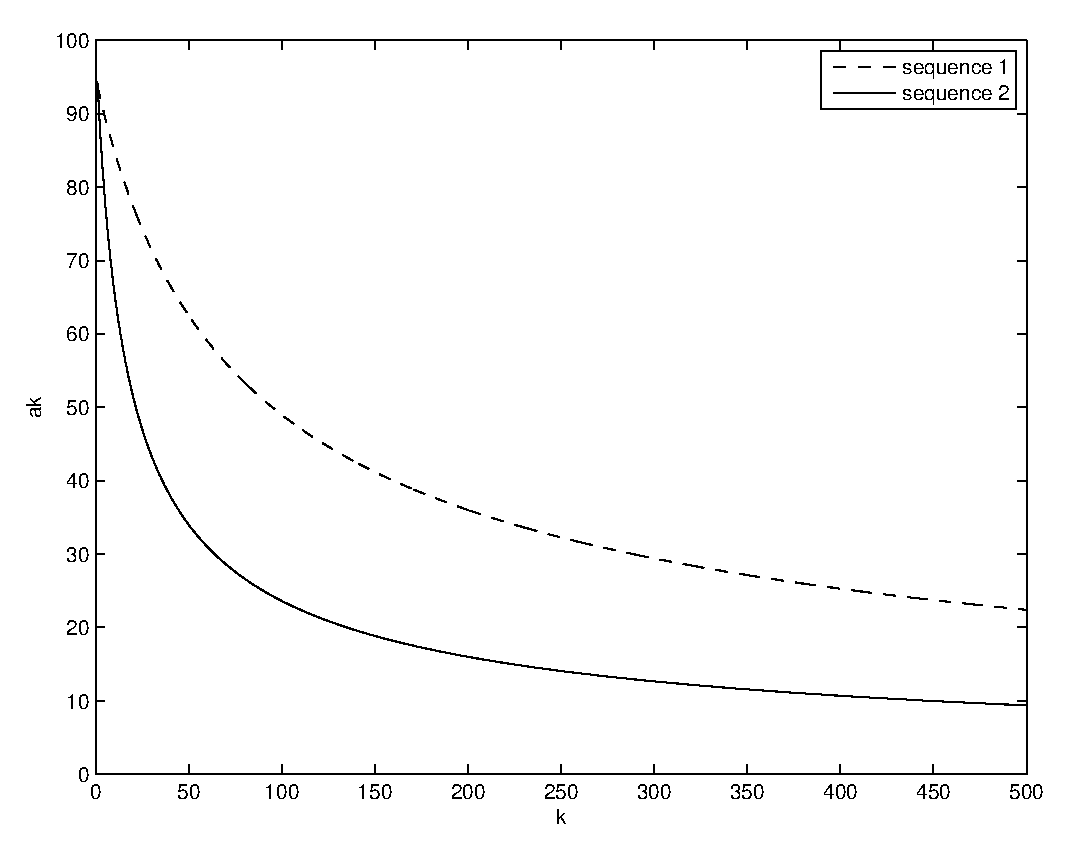
\includegraphics[width=8cm]{ak.eps}
\caption{Sequence 1: $a = 1000$, $A = 50$, $\alpha = 0.602$.
Sequence 2: $a = 400$, $A = 10$, $\alpha = 0.602$. Both sequences
start with the same step size, but sequence 2 decays much
faster.}\label{fig:ak}
\end{figure}
The parameters $\alpha$ and $A$ define the decay slope of the
function. For the parameter $\alpha$ we recommend the value 0.6.
For $A$, use something in the order of 50:
\begin{quote}
\texttt{(SP\_alpha 0.6)} \\
\texttt{(SP\_A 50.0)}
\end{quote}
This leaves the parameter $a$, called \texttt{SP\_a} in \elastix,
as the most important parameter to tune. And it is an important
parameter, it can mean success for a good choice and failure if
not! If $a$ is set too high, the iterative solving algorithm
(\ref{eq:RM}) becomes unstable, and you may deform your image
beyond recognition. If $a$ is set too low, you will never make it
to the optimum, or may get stuck in a very small nearby local
optimum. Figure~\ref{fig:stepsize} illustrates this.
\begin{figure}
\centering
\subfigure[]{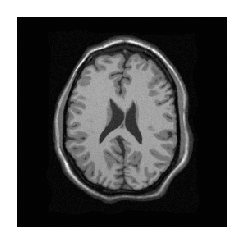
\includegraphics[width=4cm]{fixed.eps}}\label{sfig:stepsize:fixed}
\subfigure[]{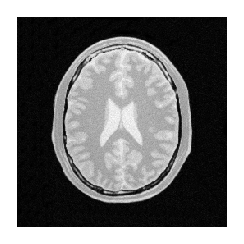
\includegraphics[width=4cm]{moving.eps}}\label{sfig:stepsize:moving} \\
\subfigure[]{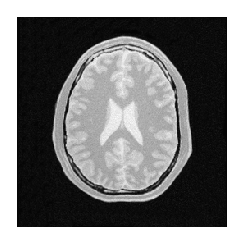
\includegraphics[width=4cm]{a320.eps}}\label{sfig:stepsize:a320}
\subfigure[]{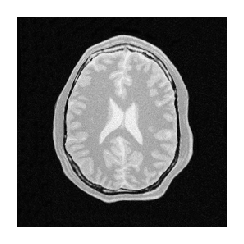
\includegraphics[width=4cm]{a3200.eps}}\label{sfig:stepsize:a3200}
\subfigure[]{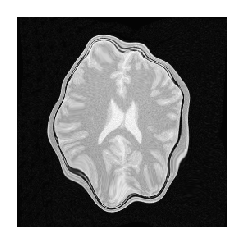
\includegraphics[width=4cm]{a32000.eps}}\label{sfig:stepsize:a32000}
\caption{The effect of the choice of the step size $a$
(\texttt{SP\_A}). This example can be downloaded from the
\elastix\ website. (a) the fixed image, (b) the moving image.
(c)-(e) show the registered images, with (c) $a = 320$ is too
small, (d) $a = 3200$ as in the downloadable example is good, (e)
$a = 32000$ is too large.} \label{fig:stepsize}
\end{figure}
A good choice for $a$ is dependent on the cost function that is used
for registration: the $a$ that will give you a good result for SSD
is not the same as the one that gives a good result for MI. Finally,
$a$ also depends on the amount of deformation that you expect
between the fixed and the moving image. So again, recommendations
are hard to give. In general we advise you to think in orders of
magnitude, if $a = 10$ is too small, try $a = 100$ and not $a = 11$.
For mutual information, normalised correlation coefficient, and
normalised mutual information, you could start around $a = 1000$.
For the mean squared difference metric you could try something
smaller than 1. If $a$ is chosen way too big, you may encounter the
error message ``Too many samples map outside moving image buffer''.
This error may have other causes as well though. The FAQ at the
\elastix\ website gives more information on this error message.

For every resolution you could specify a different value of
\texttt{SP\_a}, but it might be easier to start with the same
value for every resolution.
\begin{quote}
\texttt{(SP\_a 1000.0 1000.0 1000.0)}
\end{quote}
or, equivalently:
\begin{quote}
\texttt{(SP\_a 1000.0)}
\end{quote}

The last important option related to the optimiser is the maximum
number of iterations:
\begin{quote}
\texttt{(MaximumNumberOfIterations 500)}
\end{quote}
which is, in the case of \texttt{StandardGradientDescent}, not only
the maximum, but also the minimum, since there is no other stopping
condition implemented for this optimiser. In general, the more
iterations, the better the registration result. But, of course, more
iterations take more time. A value of 500 is a good start. Use 2000
if computation time is not such an issue. You may try to go down to
200 iterations if you are in a hurry. For small 2D images, and rigid
registration, even less iterations may suffice. A side benefit of
using more iterations is that a wider range of \texttt{SP\_a} gives
good results. Tuning \texttt{SP\_a} then becomes easier.

A relatively new development is that of an adaptive stochastic
gradient descent algorithm \cite{Klein09}, which does not require
tuning $a$. This optimiser is covered in Chapter \ref{chp:advanced}.

\subsection{Image pyramids}\label{sec:pyramidtuning}

The \texttt{FixedImagePyramid} and the \texttt{MovingImagePyramid}
have identical options. What is said below about the
FixedImagePyramid works similarly for the MovingImagePyramid.

Use the \texttt{FixedSmoothingImagePyramid}, since it will not throw
away valuable information, and since you are not using the
\texttt{FullSampler} anyway, down-sampling will not save you any
time. It may consume quite some memory though for large images and
many resolution levels. Two parameters have to be set to define the
multi-resolution strategy: the number of resolutions
(\texttt{NumberOfResolutions}) and the specific down-sampling
schedule that is used in each resolution
(\texttt{FixedImagePyramidSchedule}). If you only set the
\texttt{NumberOfResolutions}, a default schedule will be used that
smoothes the fixed image by a factor of 2 in each dimension,
starting from $\sigma = 0.5$ in the last resolution. That schedule
is usually fine. In case you have highly anisotropic data, you might
want to blur less in the direction of the largest spacing.

In general 3 resolutions is a good starting point. If the fixed and
moving image are initially far away, you can increase the number of
resolution levels to, say, 5 or 6. This way the images are more
blurred and more attention is paid to register large, dominant
structures.

The pyramid schedule defines the amount of blurring (and
down-sampling in case a \texttt{FixedRecursiveImagePyramid} is used),
in each direction $x,y,z$ and for each resolution level. It can be
specified as follows:
\begin{quote}
\texttt{(NumberOfResolutions 4)} \\
\texttt{(FixedImagePyramidSchedule 8 8 4 4 2 2 1 1)}
\end{quote}
In this example 4 resolutions for a 2D image are used. At
resolution level 0 the image is blurred with $\sigma = 8/2$ voxels
in each direction ($\sigma$ is half the pyramid schedule value).
At level 1 $\sigma = 4/2$ is used, and finally at the last level,
level 4, the original images are used for registration. Specifying
the fixed and moving image pyramids with an identical schedule can
be done with one command:
\begin{quote}
\texttt{(ImagePyramidSchedule 4 4 2 2 2 1 1 1 1)}
\end{quote}
for a 3D image with 3 resolution levels, where less smoothing is
performed in the $z$-direction.

\section{Masks}

Sometimes you are specifically interested in aligning only a part of
the image. A possibility to focus on this part is to crop the image.
Cropping, however, restricts the region of interest (ROI) to be a
square (2D) or cube (3D) only. If you need an irregular shaped ROI,
you can use masks. A mask is a binary image, filled with 0's and 1's.
If you use a mask, you only perform registration on the part of the
image that is within the masks, i.e. where the mask has 1's.

You can/should use a mask
\begin{itemize}
\item when your image contains an artificial edge that has no real meaning.
The registration might be tempted to align these artificial edges,
thereby neglecting the meaningful edges. The conic beam edge in
ultrasound images is an example of such an artificial edge.

\item when the image contains structures in the neighbourhood
of your ROI that may influence the registration within your ROI. This
is for example the case when matching lung data. Usually, you are
interested in the lungs, and not if the rib cage is well aligned.
However, the ribs are structures that for example in CT can have a
strong influence on the similarity metric, especially if you use the
SSD metric. In that case, the rib cage may be well aligned at the
cost of vessels structures near the border of the lung with the rib
cage. In this case it will help you if you use a dilated lung
segmentation as a mask.
\end{itemize}

Masks can be used both for the fixed and the moving image. A fixed
image mask is sufficient to focus the registration on a ROI, since
samples are drawn from the fixed image. You only want to use a
mask for the moving image when your moving image contains nonsense
grey values near the ROI.

In case you are using a mask to prevent bad karma from an artificial
edge, you also need to set the parameter:
\begin{quote}
\texttt{(ErodeMask "true")}
\end{quote}
If not, then when performing multi-resolution, information from the
artificial edge will flow into you ROI due to the smoothing step. In
case the edge around your ROI is meaningful, e.g. in the lung
example, you should set it to false, because this edge will help to
guide the registration.

A common exception that \elastix\ throws when drawing samples is:
``Could not find enough image samples within reasonable time.
Probably the mask is too small.'' The probable cause for this is
that your fixed image mask is too small. See the FAQ for more
information.

\section{Trouble shooting}

\subsection{Common errors}

Some common sources of confusion and questions have been gathered in
a FAQ, which can be found at
\begin{quote}
\url{http://elastix.isi.uu.nl/FAQ.php}
\end{quote}

\subsection{Bad initial alignment}

When the initial alignment between two images is very off, you cannot
start a nonrigid registration. And sometimes it can be a hassle to
get it right. What factors can help to get it right?

\begin{itemize}
\item Start with a transformation with a low degree of freedom,
i.e. the translation, rigid, similarity or affine transform.
Sometimes the images are really far off, and have no overlap to
begin with (NB: the position of images in physical space is
determined by the origin and voxel spacing; see
Section~\ref{sec:comp:image}). A solution is then to add the
following line to your parameter file:
\begin{quote}
  \texttt{(AutomaticTransformInitialization "true")}
\end{quote}
which aligns the centres of the fixed and moving image.

\item You need a good multi-resolution strategy, i.e.
quite a bit of resolution levels. This way a lot of smoothing is
going on, blurring away all the details and thereby focussing the
registration on the major structures.

\item Use more iterations.

\item Take larger steps. Set the
parameter $a$ so high that the translation component of the
transformation takes a step of several voxels in each iteration, up
to 10. Maybe it will work, and in that case you will get alignment
pretty quick, but the step size $a$ is still large, so you
immediately jump away from alignment again. If that happens, you
should let the sequence $a_k = a / (A+k)^{\alpha}$ decay relatively
fast. This can be achieved by setting both $a$ and $A$ a bit lower,
see Figure \ref{fig:ak}.

\item In case you need to find a large rotation, you might want to
take larger steps for the rotation, but not for the translation.
This can be achieved by modifying the scales parameter, see
Section \ref{sec:transformtuning}:
\begin{quote}
\texttt{(Scales 10000.0)}
\end{quote}
You can set it lower to take larger rotation steps. If it is set
to 1.0 you take as large steps for the rotation as for the
translation (but the rotation is defined in radials). If you set
it really high ($> 10^6$) you won't rotate at all. You probably
don't need to go lower than 1000.0. Note that the
\texttt{AutomaticScalesEstimation} option usually works fine, so
specifying \texttt{Scales} is not necessary.

\end{itemize}

\subsection{Memory consumption}\label{ssec:tut:memory}

The typical size of clinical images increases as a function of time.
Therefore, memory efficiency will become more of an issue. \elastix\
consumes $\approx$ 100 MB of memory for small images, for larger
image pairs ($256^3$) and some common components, consumption can be
about 1 - 1.5 GB. With very large images ($400^3$ and above) memory
consumption can rise above the 2 GB limit of most Windows systems.
What to do with large images?
\begin{itemize}
\item Buy yourself a brand new computer with a lot of memory. Make
sure that this computer is 64 bit, otherwise you cannot address this
much memory. Also make sure that your operating system supports 64
bit.

\item Images in \elastix\ are internally by default represented as a bunch of
voxels of floating type. You can modify this to short images:
\begin{quote}
\texttt{(FixedInternalImagePixelType "short")} \\
\texttt{(MovingInternalImagePixelType "short")}
\end{quote}
This way you save half the amount of memory that is used to store the
fixed and moving images, and their multi-resolution pyramids. This
will come at the cost of a loss of precision, but may not be that
harmful. This option is useful both for \elastix\ and \transformix.

\item Change the interpolator that is used during registration. By default a B-spline
interpolator is used, which stores a coefficient image internally in
double type. You can also specify a float version:
\begin{quote}
\texttt{(Interpolator "BSplineInterpolatorFloat")}
\end{quote}
which saves you another bit of memory the size of a short image.
This option is useful for \elastix\ only. To save even more
memory, use the \texttt{LinearInterpolator}. This may change the
results a little though, because of its different method to
compute image derivatives.

\item Change the interpolator that is used when resampling an image:
\begin{quote}
\texttt{(ResampleInterpolator "FinalBSplineInterpolatorFloat")}
\end{quote}
This option is useful both for \elastix\ and \transformix. However,
for \elastix\ it will only save you some memory at the very end of
the registration.

\item Use downsampled images during the registration. This probably
will not effect the registration accuracy too much. After
registration you can apply the resulting transformation to the
original full size moving image, using \transformix. See the FAQ for
more information.

\end{itemize}

%\section{Example}
%
%Step-by-step example where we give a look into our head, what magical
%thoughts we think when tuning the registration.

%%%%%%%%%%%%%%%%%%%%%%%%%%%%%%%%%%%%%%%%%%%%%%%%%%%%%%%%%%%%%%%%%%%%%%%%%%%%%%%%%%%%%%%%%%%%

\chapter{Advanced topics}\label{chp:advanced}

\section{Metrics}

\subsection{Image registration with multiple metrics and/or images}

Up till now we viewed image registration as the problem of finding
the spatial relation between one fixed image and one moving image,
using one similarity metric to define the fit. Sometimes, it is
desirable to combine multiple metrics, or multiple fixed and moving
images, or both. All these three generalisations are available in \elastix:
\begin{description}
\item[multi-metric] In this case the registration cost function is defined
as:
\begin{align}
\CC(\vTm; I_F, I_M) &= \frac{1}{\sum_{i=1}^N \omega_i} \sum_{i=1}^N
\omega_i \CC_i(\vTm; I_F, I_M),
\end{align}
with $\omega_i$ the weights. This way the same fixed and moving
image is used for every sub-metric $\CC_i$. This way one can for
example simultaneously optimise the SSD and MI during a
registration.

\elastix\ should be called like:
\begin{quote}
\texttt{elastix -f fixed.ext -m moving.ext -out outDir -p parameterFile.txt}
\end{quote}

\item[multi-image] In this case the registration cost function is defined
as:
\begin{align}
\CC(\vTm; I_F, I_M) &= \frac{1}{\sum_{i=1}^N \omega_i} \sum_{i=1}^N
\omega_i \CC(\vTm; I_F^i, I_M^i).
\end{align}
This way one can simultaneously register all channels of
multi-spectral input data, using a single type of cost function for
all channels.

\elastix\ should be called like:
\begin{quote}
\texttt{elastix -f0 fixed0.ext -f1 fixed1.ext -f<>... -m0
moving0.ext
 -m1 moving1.ext -m<>... -out outDir -p parameterFile.txt}
\end{quote}

\item[both] In this case the registration cost function is defined
as:
\begin{align}
\CC(\vTm; I_F, I_M) &= \frac{1}{\sum_{i=1}^N \omega_i} \sum_{i=1}^N
\omega_i \CC_i(\vTm; I_F^i, I_M^i).
\end{align}
This is the most general way of registration supported by \elastix.
This will make it possible for example to register two lung CT data
sets with MI, while simultaneously registering the fissure
segmentations with the kappa statistic. The two may help each other
in getting a better registration compared to only using a single channel.
\end{description}

All three scenarios use the multi-metric registration method, which
is selected in the parameter file with:
\small
\begin{verbatim}
(Registration "MultiMetricMultiResolutionRegistration")
\end{verbatim}
\normalsize Other parts of the parameter file should look like:
\small
\begin{verbatim}
(FixedImagePyramid "FixedSmoothingImagePyramid" "FixedSmoothingImagePyramid" ...)
(MovingImagePyramid "MovingSmoothingImagePyramid" "MovingSmoothingImagePyramid" ... )
(Interpolator "BSplineInterpolator" "BSplineInterpolator" ...)
(Metric "AdvancedMattesMutualInformation" "AdvancedMeanSquareDifference" ...)
(ImageSampler "RandomCoordinate" "RandomCoordinate" ...)

(Metric0Weight 0.125)
(Metric1Weight 0.125)
(Metric2Weight 0.125)
etc
\end{verbatim}
\normalsize

Another way of registering multi-spectral data is to use the
$\alpha$-mutual information measure, described below.

\subsection{Additional metrics}

Some more advanced metrics, not found in the ITK, are available in
\elastix:
\begin{description}
\item[Mutual information with rigidity penalty] This metric computes the combined
cost function
\begin{align}
\CC &= \mathit{MI}(\vTm;I_F,I_M) + \omega
\mathcal{P}^{\mathrm{rigid}}(\vTm;I_M)
\end{align}
with $\mathcal{P}^{\mathrm{rigid}}$ the rigidity penalty term
described in \cite{Staring07}. It is specified in the parameter file
with: \small
\begin{verbatim}
(Metric "MattesMutualInformationWithRigidityPenalty")
// normal Mattes MI parameters
...

// Rigidity penalty parameters:
(RigidityPenaltyWeight 0.1)
(LinearityConditionWeight 10.0)
(OrthonormalityConditionWeight 1.0)
(PropernessConditionWeight 100.0)
(MovingRigidityImageName "movingRigidityImage.mhd")
\end{verbatim}
\normalsize A complete list of the available parameters can be found at
\url{http://elastix.isi.uu.nl/doxygen/a00056.html}. See also
Section~\ref{sec:penaltyterms}.

\item[$\alpha$-mutual information] This metric computes true multi-channel
$\alpha$-mutual information. It does not use high-dimensional joint
histograms, but instead relies on $k$-nearest neighbour graphs to
estimate $\alpha$-MI. Details can be found in \cite{Staring09}. It
is specified in the parameter file with: \small
\begin{verbatim}
(Registration "MultiResolutionRegistrationWithFeatures")
(FixedImagePyramid "FixedSmoothingImagePyramid" "FixedSmoothingImagePyramid")
(MovingImagePyramid "MovingSmoothingImagePyramid" "MovingSmoothingImagePyramid")
(Interpolator "BSplineInterpolator" "BSplineInterpolator")
(Metric "KNNGraphAlphaMutualInformation")
(ImageSampler "MultiInputRandomCoordinate")

// KNN specific
(Alpha 0.99)
(AvoidDivisionBy 0.0000000001)
(TreeType "KDTree")
(BucketSize 50)
(SplittingRule "ANN_KD_STD")
(ShrinkingRule "ANN_BD_SIMPLE")
(TreeSearchType "Standard")
(KNearestNeighbours 20)
(ErrorBound 10.0)
\end{verbatim}
\normalsize A complete list of the available parameters can be found
at \url{http://elastix.isi.uu.nl/doxygen/a00053.html}.
\end{description}

\subsection{Penalty terms}\label{sec:penaltyterms}

This paragraph requires extension and modification.

In order to regularise the transformation $\vT_{\vmu}$ often a
penalty term $\mathcal{P}(\vmu)$ is added to the cost function, so
it becomes:
\begin{align}
\mathcal{C} &= \omega_1 \mathcal{S} + \omega_2 \mathcal{P},
\end{align}
where $\omega_1, \omega_2$ user-defined constants that weigh
similarity against regularity.

Penalty term are often based on the first or second order spatial
derivatives of the transformation. For example the bending energy of
the transformation, which is arguably the most common penalty term,
is defined in 2D as:
\begin{align}
\mathcal{P}_{\mathrm{BE}}(\vmu) &= \frac{1}{P} \sum_{\vxt[i]}
\left\| \frac{\partial^2 \vT}{\partial \vx \partial \vx^T}(\vxt[i])
\right\|_F^2 \\
&= \frac{1}{P} \sum_{\vxt[i]} \sum_{j = 1}^2 \left( \frac{\partial^2
T_j}{\partial x_1^2}(\vxt[i]) \right)^2  + 2 \left( \frac{\partial^2
T_j}{\partial x_1 \partial x_2}(\vxt[i]) \right)^2 + \left(
\frac{\partial^2 T_j}{\partial x_2^2}(\vxt[i]) \right)^2,
\end{align}
where $P$ is the number of points $\vxt[i]$, and the tilde denotes
the difference between a variable and a given point over which a
term is evaluated.

The derivative of the similarity measure usually involves
computation of the spatial derivative of the moving image:
$\D{I_M}{\vx}$, and the derivative of the transformation to its
parameters: $\D{\vT}{\vmu}$. In the ITK the last derivative is
implemented using $\texttt{transform->GetJacobian()}$, i.e. the
derivative to the transformation parameters $\vmu$ is referred to as
`Jacobian'.

Penalty terms usually consist of the first and second order
\emph{spatial} derivatives of the transformation, i.e.
$\D{\vT}{\vx}$ and $\Dd{\vT}{\vx}{\vx^T}$. We will refer to these
derivatives as the `SpatialJacobian' and the `SpatialHessian' to
clearly distinguish between these derivatives and the `Jacobian'. In
order to apply the gradient descent optimisation routine
(\ref{eq:gd}), (\ref{eq:RM}), we additionally need the derivatives
$\D{}{\vmu} \D{\vT}{\vx}$ and $\D{}{\vmu} \Dd{\vT}{\vx}{\vx^T}$.
These we call the `JacobianOfSpatialJacobian' and
`JacobianOfSpatialHessian', respectively.

The transform class as defined in the ITK does not support the computation of
spatial derivatives $\partial \vT / \partial \vx$ and $\partial^2 \vT /
\partial \vx^2$, and their derivatives to $\vmu$. Initially, we created
non-generic classes that combine MI and the mentioned penalty terms
specifically (the \texttt{MattesMutualInformationWithRigidityPenalty} component
in \elastix). Recently, however, we created a more advanced version of the ITK
transform that does implement these spatial derivatives. Additionally, we
created a bending energy regularisation class that takes advantage of these
functions. We also reimplemented the rigidity penalty term.

This all means that it is possible in \elastix\ to combine any similarity
metric with any of the available penalty terms (currently the bending energy
and the rigidity penalty term).

\subsection{DisplacementMagnitudePenalty: inverting transformations}

The \texttt{DisplacementMagnitudePenalty} is a cost function that
penalises $||\vTm(\vx)-\vx||^2$. You can use this to invert
transforms, by setting the transform to be inverted as an initial
transform (using \texttt{-t0}), setting
\texttt{(HowToCombineTransforms "Compose")}, and running \elastix\
with this metric. After that you can manually set the initial
transform in the last parameter file to
\texttt{"NoInitialTransform"}, and voila, you have the inverse
transform! Strictly speaking, you should then also change the
Size/Spacing/Origin/Index settings to match that of the moving
image. Select it with:
\begin{verbatim}
(Metric "DisplacementMagnitudePenalty")
\end{verbatim}
Note that inverting a transformation becomes conceptually very similar to
performing an image registration in this way. Consequently, the same choices
are relevant: optimisation algorithm, multiresolution etc...

\section{Image samplers}

\begin{description}
\item[RandomSparseMask] This variant of the random sampler is useful if the
    fixed image mask is sparse (i.e. consists of many zeros).
\end{description}

\section{Transforms}

\begin{description}
\item[DeformationFieldTransform] This transform serves as a wrapper around
    existing deformation field vector images. It computes the
    transformation by interpolating the deformation field image. The
    relevant tags in the transform parameter file are as follows:
\begin{verbatim}
(Transform "DeformationFieldTransform")
(DeformationFieldFileName "deformationField.mhd")
(DeformationFieldInterpolationOrder 1)
(NumberOfParameters 0)
\end{verbatim}
The deformation field image's pixel type should be a vector of
\texttt{float} elements. It could be a deformation field that is the
result of \texttt{transformix -def all} for example! Since this
transform does not have any parameters (the $\vmu$ has zero length),
it makes no sense to use it for registration. It can just be used as
an initial transformation (supplied by the option \texttt{-t0}) or
as input for \transformix.

\item[SplineKernelTransform] As an alternative to the B-spline transform,
    \elastix\ includes a the \texttt{SplineKernelTransform}, which
    implements a thin-plate spline type of transform. This transformation
    requires a list of fixed image landmarks (control points) to be
    specified, by means of an input points file which has the same format
    as the \texttt{-def} file used by \transformix\
    (Section~\ref{sec:calltransformix}. See the \texttt{doxygen}
    documentation on the website for a list of its parameters.

\item[WeightedCombinationTransform] This is a transformation that is
    modelled as a weighted combination of user-specified transformations:
    $\vTm(\vx) = \sum_i w_i \vT_i(\vx)$. The weights $w_i$ form the
    parameter vector $\vmu$. The sub-transforms $\vT_i(\vx)$ may for
    example follow from a statistical deformation model, obtained by
    principal component analysis. See the \texttt{doxygen} documentation on
    the website for a list of its parameters.

\item[BSplineDeformableTransformWithDiffusion] This transform implements
    the work described in \cite{Staring07a}.
\end{description}

\section{Optimisation methods}

\begin{description}
\item[AdaptiveStochasticGradientDescent] This optimizer is very similar to
    the StandardGradientDescent, but implements an adaptive step size
    mechanism and estimates a proper initial value for \texttt{SP\_a}. See
    \cite{Klein09} for more details. In practice this optimizer works in
    many applications with its default settings. Only the number of
    iterations must be specified by the user:
\begin{verbatim}
(Optimizer "AdaptiveStochasticGradientDescent")
(MaximumNumberOfIterations 500)
(SigmoidInitialTime 4.0)
(MaximumStepLength 1.0)
\end{verbatim}
The last two options are not mandatory. \texttt{SigmoidInitialTime}
corresponds to $t_0$ in the article; its default value is 0. The
\texttt{MaximumStepLength} corresponds to $\delta$ in the article; its
default value equals the average voxel spacing of fixed and moving image.

\item[Conjugate gradient]
---ConjugateGradientFRPR

\item[CMAEvolutionStrategy]

\item[FiniteDifferenceGradientDescent]

\item[Full search]

\item[Quasi Newton]

%\item[Preconditioned Stochastic Gradient Descent

\item[RegularStepGradientDescent]
---RSGDEachParameterApart

\item[SimultaneousPerturbation]
\end{description}


%%%%%%%%%%%%%%%%%%%%%%%%%%%%%%%%%%%%%%%%%%%%%%%%%%%%%%%%%%%%%%%%%%%%%%%%%%%%%%%%%%%%%%%%%%%%

\chapter{Developers guide}\label{chp:develop}

%
\section{Setup of the code}

The \elastix\ source code consists roughly of two layers, both
written in C++: A) ITK-style classes that implement image
registration functionality, and B) \elastix\ wrappers that take care
of reading and setting parameters, instantiating and connecting
components, saving (intermediate) results, and similar
`administrative' tasks. The modular design enables adding new
components, without changing the \elastix\ core. Adding a new
component starts by creating the layer A class, which can be
compiled and tested independent of layer B. Subsequently, a small
layer B wrapper needs to be written, which connects the layer A
class to the other parts of \elastix.

The image samplers, for example, are implemented as ITK classes that
all inherit from a base class \texttt{itk::ImageSamplerBase}. These
can be found in \texttt{src/Common/ImageSamplers}. So, this is
``layer A'' in \elastix. For each sampler (random, grid, full... ) a
wrapper is written, located in
\texttt{src/Components/ImageSamplers}, which takes care of
configuring the sampler before each new resolution of the
registration process. This is ``layer B'' of \elastix.

\subsection{Directory structure}

\begin{itemize}
\item dox
\item src/Common: itk classes. layer A stuff.
\item src/Core: this is the main \elastix\ kernel, responsible for the
    execution flow, connecting the classes, reading parameters etc.
\item src/Components: this directory contains the components and their
    \elastix\ wrappers (layer B)
\end{itemize}

%\subsection{\elastix\ execution flow}
%\begin{enumerate}
%\item elastix.cxx
%\item ElastixMain
%\item ElastixTemplate (Run)
%\item concept of observer/command structure;
%    overzicht van al dit soort functies:
%    \begin{itemize}
%    \item BeforeAll
%    \item BeforeRegistratioin
%    \item BeforeEachResolution
%    \item AfterEachResolution
%    \item AfterEachIteration
%    \item AfterRegistration
%    \end{itemize}
%\end{enumerate}
%
%\subsection{\transformix\ execution flow}
%\begin{enumerate}
%\item transformix.cxx
%\item TransformixMain
%\item ElastixTemplate (RunTransformix)
%\item overzicht van al dit soort functies:
%    \begin{itemize}
%    \item BeforeAll
%    \item ApplyTransform
%    \item ...
%    \end{itemize}
%\end{enumerate}
%
%\subsection{External packages}
%
%\elastix\ uses a few external packages, which are included in the
%source.
%
%\begin{itemize}
%\item Parameter file parser
%\item xout
%\item ANN license! used for a not yet released component.
%\end{itemize}

\section{Functional differences with the ITK}

%Although \elastix\ is based on the ITK registration framework, it
%implements several functional enhancements.
%
%- AdvancedImageToImageMetric: ImageSampler's, ...
%
%- Advanced transformation, .....

A large part of the \elastix\ code is based on the ITK
\cite{ITKSoftwareGuideSecondEdition}. The use of the ITK implies
that the low-level functionality (image classes, memory allocation
etc.) is thoroughly tested. Naturally, all image formats supported
by the ITK are supported by \elastix\ as well. The C++ source code
can be compiled on multiple operating systems (Windows XP, Linux,
Mac OS X), using various compilers (MS Visual Studio up to version
2008, GCC up to version 4.3), and supports both 32 and 64 bit
systems. In addition to the existing ITK image registration classes,
\elastix\ implements new functionality. The most important
enhancements are listed in Table \ref{table:extras}.

\begin{table}
\centering
\begin{tabular}{p{30pc}}
\toprule \toprule
\begin{list}{\labelitemi}{\leftmargin=1em}
\item A modular framework for sampling strategies.

\item Several new optimisers: Kiefer-Wolfowitz, Robbins-Monro,
adaptive stochastic gradient descent, evolutionary strategy.

\item Complete rework of existing ITK optimisers, adding more user
control and better error handling: quasi-Newton, nonlinear conjugate
gradient.

\item Several new or more flexible cost functions: (normalised) mutual
information, implemented with Parzen windowing similar to
\cite{ThevenazEA00a}, multifeature $\alpha$-mutual information,
bending energy penalty term, rigidity penalty term.

\item The ability to concatenate any number of geometric
transformations.

\item The transformations support computation of not only
$\partial \vT / \partial \vmu$, but also of spatial derivatives
$\partial \vT / \partial \vx$ and $\partial^2 \vT / \partial \vx^2$,
and their derivatives to $\vmu$, frequently required for the
computation of regularisation terms. Additionally, the compact
support of certain transformations is integrated more generally.

\item Linear combinations of cost functions, instead of just a single cost
function.

\item A Gaussian pyramid without downsampling.
\end{list}\\
 \bottomrule \bottomrule
\end{tabular}
\caption{The most important enhancements and additions in \elastix,
compared to the ITK.}\label{table:extras}
\end{table}


%%- registration classes: what's the difference? Should we just file a
%bug fix?

\section{Creating new components}

If you want to create your own component, it is natural to start
writing the layer A filter, without bothering about \elastix. The
layer A filter should implement all basic functionality,

You can simply extract the ImageSampler directory from \elastix\ and
make a small test program that reads an image, runs the sampler, and
verifies its output. Once you got the new sampler to work, it is
trivial to write the layer B wrapper in \elastix\ (some copy-paste
from existing samplers).


%%%%%%%%%%%%%%%%%%%%%%%%%%%%%%%%%%%%%%%%%%%%%%%%%%%%%%%%%%%%%%%%%%%%%%%%%%%%%%%%%%%%%%%%%%%%

\appendix

\chapter{Example parameter file}\label{chp:ExampleParam}

\small
\begin{verbatim}
//ImageTypes
(FixedInternalImagePixelType "float")
(FixedImageDimension 2)
(MovingInternalImagePixelType "float")
(MovingImageDimension 2)

//Components
(Registration "MultiResolutionRegistration")
(FixedImagePyramid "FixedRecursiveImagePyramid")
(MovingImagePyramid "MovingRecursiveImagePyramid")
(Interpolator "BSplineInterpolator")
(Metric "AdvancedMattesMutualInformation")
(Optimizer "StandardGradientDescent")
(ResampleInterpolator "FinalBSplineInterpolator")
(Resampler "DefaultResampler")
(Transform "EulerTransform")

// ********** Pyramid

// Total number of resolutions
(NumberOfResolutions 3)


// ********** Transform

//(CenterOfRotation 128 128) center by default
(AutomaticTransformInitialization "true")
(AutomaticScalesEstimation "true")
(HowToCombineTransforms "Compose")


// ********** Optimizer

// Maximum number of iterations in each resolution level:
(MaximumNumberOfIterations 300 300 600)

//SP: Param_a in each resolution level. a_k = a/(A+k+1)^alpha
(SP_a 0.001)

//SP: Param_alpha in each resolution level. a_k = a/(A+k+1)^alpha
(SP_alpha 0.602)

//SP: Param_A in each resolution level. a_k = a/(A+k+1)^alpha
(SP_A 50.0)


// ********** Metric

//Number of grey level bins in each resolution level:
(NumberOfHistogramBins 32)
(FixedKernelBSplineOrder 1)
(MovingKernelBSplineOrder 3)


// ********** Several

(WriteTransformParametersEachIteration "false")
(WriteTransformParametersEachResolution "false")
(ShowExactMetricValue "false")
(ErodeMask "true")


// ********** ImageSampler

// Number of spatial samples used to compute the
// mutual information in each resolution level:
(ImageSampler "RandomCoordinate")
(NumberOfSpatialSamples 2048)
(NewSamplesEveryIteration "true")


// ********** Interpolator and Resampler

//Order of B-Spline interpolation used in each resolution level:
(BSplineInterpolationOrder 1)

//Order of B-Spline interpolation used for applying the final deformation:
(FinalBSplineInterpolationOrder 3)

//Default pixel value for pixels that come from outside the picture:
(DefaultPixelValue 0)
\end{verbatim}
\normalsize

%%%%%%%%%%%%%%%%%%%%%%%%%%%%%%%%%%%%%%%%%%%%%%%%%%%%%%%%%%%%%%%%%%%%%%%%%%%%%%%%%%%%%%%%%%%%

\chapter{Example transform parameter file}\label{chp:ExampleTransformParam}

\small
\begin{verbatim}
(Transform "EulerTransform")
(NumberOfParameters 3)
(TransformParameters -0.000000 -4.564513 -2.091174)
(InitialTransformParametersFileName "NoInitialTransform")
(HowToCombineTransforms "Compose")

// Image specific
(FixedImageDimension 2)
(MovingImageDimension 2)
(FixedInternalImagePixelType "float")
(MovingInternalImagePixelType "float")
(Size 256 256)
(Index 0 0)
(Spacing 1.0000000000 1.0000000000)
(Origin 0.0000000000 0.0000000000)

// EulerTransform specific
(CenterOfRotationPoint 128.0000000000 128.0000000000)

// ResampleInterpolator specific
(ResampleInterpolator "FinalBSplineInterpolator")
(FinalBSplineInterpolationOrder 3)

// Resampler specific
(Resampler "DefaultResampler")
(DefaultPixelValue 0.000000)
(ResultImageFormat "mhd")
(ResultImagePixelType "short")
\end{verbatim}
\normalsize

%%%%%%%%%%%%%%%%%%%%%%%%%%%%%%%%%%%%%%%%%%%%%%%%%%%%%%%%%%%%%%%%%%%%%%%%%%%%%%%%%%%%%%%%%%%%

\chapter{Software License} \label{chp:License}

\small
\begin{verbatim}
Overview:

Elastix was developed by Stefan Klein and Marius Staring under
supervision of Josien P.W. Pluim, initially under contract to the
Image Sciences Institute, University Medical Center Utrecht, The
Netherlands.

Elastix is distributed under the new and simplified BSD license
approved by the Open Source Initiative (OSI)
[http://www.opensource.org/licenses/bsd-license.php].

The software is partially derived from the Insight Segmentation and
Registration Toolkit (ITK), which is also distributed under the new
and simplified BSD licence. The ITK is required by Elastix for
compilation of the source code.

The copyright of the files in the Common/KNN/ann_1.1 subdirectory
is held by a third party, the University of Maryland. The ANN
package is distributed under the GNU Lesser Public Licence. Please
read the content of the subdirectory for specific details on this
third-party license.


Elastix Copyright Notice:

      Copyright (c) 2004-2010 University Medical Center Utrecht
      All rights reserved.


License:

Redistribution and use in source and binary forms, with or without
modification, are permitted provided that the following conditions
are met:

    * Redistributions of source code must retain the above copyright notice,
      this list of conditions and the following disclaimer.

    * Redistributions in binary form must reproduce the above copyright notice,
      this list of conditions and the following disclaimer in the documentation
      and/or other materials provided with the distribution.

    * Neither the name of the University Medical Center Utrecht nor the names of
      its contributors may be used to endorse or promote products derived from
      this software without specific prior written permission.

THIS SOFTWARE IS PROVIDED BY THE COPYRIGHT HOLDERS AND
CONTRIBUTORS "AS IS" AND ANY EXPRESS OR IMPLIED WARRANTIES,
INCLUDING, BUT NOT LIMITED TO, THE IMPLIED WARRANTIES OF
MERCHANTABILITY AND FITNESS FOR A PARTICULAR PURPOSE ARE
DISCLAIMED. IN NO EVENT SHALL THE COPYRIGHT OWNER OR CONTRIBUTORS
BE LIABLE FOR ANY DIRECT, INDIRECT, INCIDENTAL, SPECIAL,
EXEMPLARY, OR CONSEQUENTIAL DAMAGES (INCLUDING, BUT NOT LIMITED
TO, PROCUREMENT OF SUBSTITUTE GOODS OR SERVICES; LOSS OF USE,
DATA, OR PROFITS; OR BUSINESS INTERRUPTION) HOWEVER CAUSED AND ON
ANY THEORY OF LIABILITY, WHETHER IN CONTRACT, STRICT LIABILITY, OR
TORT (INCLUDING NEGLIGENCE OR OTHERWISE) ARISING IN ANY WAY OUT OF
THE USE OF THIS SOFTWARE, EVEN IF ADVISED OF THE POSSIBILITY OF
SUCH DAMAGE.
\end{verbatim}
\normalsize

%%%%%%%%%%%%%%%%%%%%%%%%%%%%%%%%%%%%%%%%%%%%%%%%%%%%%%%%%%%%%%%%%%%%%%%%%%%%%%%%%%%%%%%%%%%%

\newpage
\pagestyle{plain} \addcontentsline{toc}{chapter}{Bibliography}
\bibliographystyle{plainnat}
\bibliography{IEEEabrv,manual}

\end{document}
